\pagebreak
\section{3D Results}
\add[XT]{add one more section as an individual file/chapter for 2D models description.}
%\subsection{3D model results}
%\add[XT]{choose some points in the model domain like Choi 2008 did, to monitor the values changes with time (e.g. In VisIt use Query to obtain stress with time for quantatatively analyzing the model behaviors)}
Currently, we have three factors controlling the model behaviors. They are three ranges of M variation along the ridge axis (0.5$\sim$0.7; 0.5$\sim$0.8; 0.2$\sim$0.8), three functional forms of M variation (linear; sinusoidal; square root) and two types of weakening rate (Type 1 and Type 2) as described in detail in the section ``Parameters to control''. 

Generally, all models forms a median valley that deepens and widens toward the lower M side (Figure~\hyperref[fig_Results1_1]{\ref{fig_Results1_1}}) except the reference model with constant M$=0.8$ (Figure~\hyperref[fig_Results1_3]{\ref{fig_Results1_3}}). The topography oberseved in our models, to the first order, is controlled by the spatial and temporal distributions of faulting and to the second order, results from elastically deformation (e.g. The gradual deepening and widening of the median valley; The bending of the crust at the footwall side of the detatchment fault results in a domal shape of the fault interface as a mechanism for producing the dome shape of OCCs). 

The pattern of the deformation (faulting and elastic deformation) is controlled by the evolving stress in the crust in terms of its distribution and magnitude. The stress evolution is a result of the interaction processes between tectonics and magmatism. Due to constant seafloor spreading, tensional stress orthogonal to the ridge-axis in the crust keeps accummulating. At the same time, along ridge-axis varying diking partially accommodates the stress from far field extension and perturbs the homogeneity state of stress distribution along the ridge-axis. Accumulated stress will be largely released when the normal or shear failures establish.

In this ``Results'' chapter, we will first describe in detail the model behaviors of two reference models. Then, we will compare the reference model and the other data points with different setup parameters. Formation mechanism will be explained mostly in this chapter and will be further discussed and compared with nature observation in the ``Discussion'' chapter. 

\subsection{Reference models}
We consider two models as our reference models: one, M varies linearly from 0.2 to 0.8 along the ridge axis with increasing Z; two, constant M along the ridge axis as a comparison to the changing M models.

\subsubsection{M varies along the ridge-axis}

\begin{figure}[h]
  \centering
    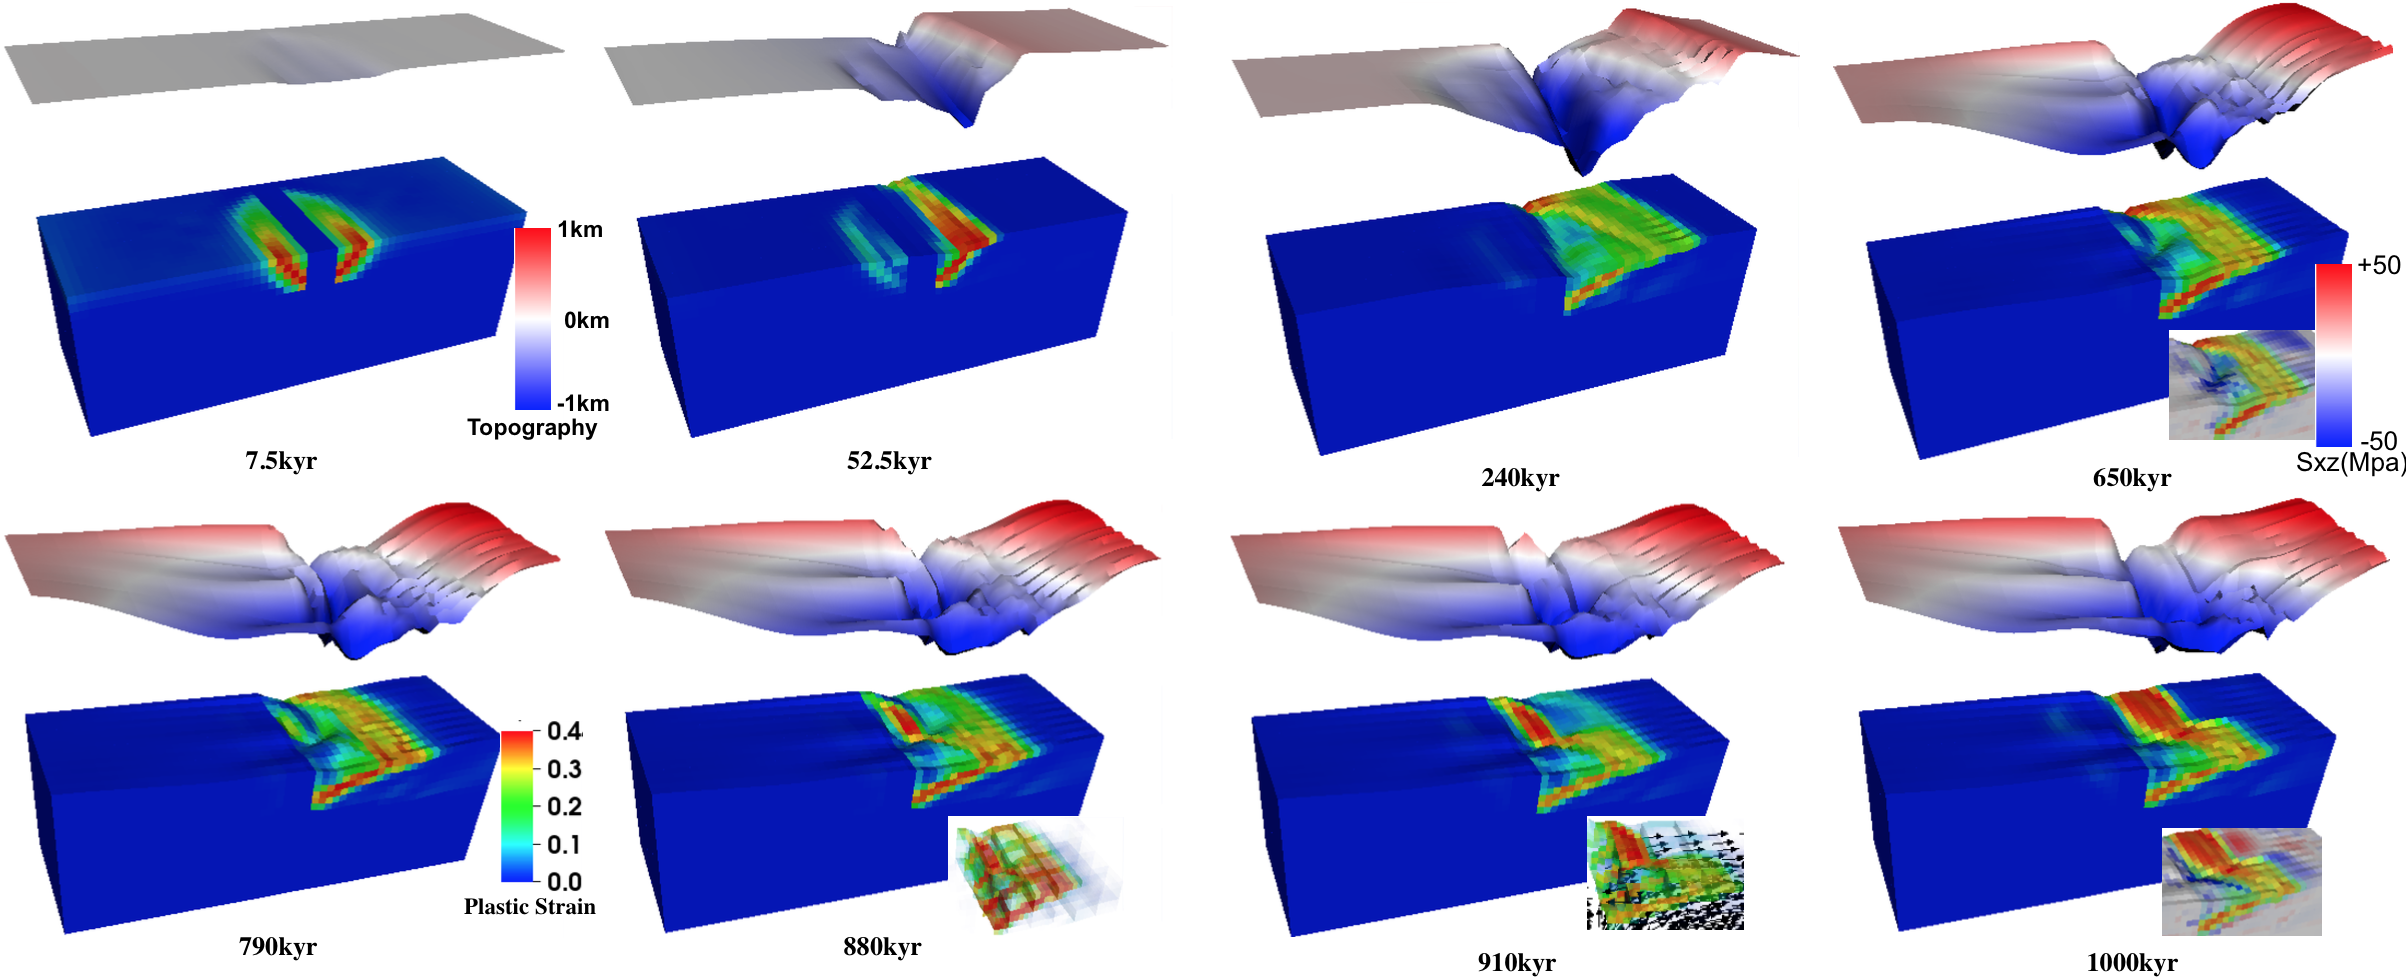
\includegraphics[width=1.0\textwidth]{fig_Results1_1.png}
  \caption{Reference model one: M linearly increases from 0.2 to 0.8 from front to back, Type one weakening (M28LinT1) (Table~\hyperref[Tab1_1]{\ref{Tab1_1}}). The top layer is the topography of the model with five times vertical exaggeration. The color scale within Figure~\hyperref[fig_Results1_1]{\ref{fig_Results1_1}.a} is for the topography. Initial seafloor is marked as a reference of zero km in height.  The green, yellow and red colors in the background of blue model domain are plastic strain. Its color scale is shown in Figure~\hyperref[fig_Results1_1]{\ref{fig_Results1_1}.e}. The number with kyr as a unit beneath each model result is the time for the model with a unit of thousands of year. The two insets in Figure~\hyperref[fig_Results1_1]{\ref{fig_Results1_1}.b} and Figure~\hyperref[fig_Results1_1]{\ref{fig_Results1_1}.d} is for stress $\sigma_{xx}$ (Sxx in the figure). Positive value (pink and red) means tension and negative (blue) is compression. The inset in Figure~\hyperref[fig_Results1_1]{\ref{fig_Results1_1}.h} is for shear stress $\sigma_{xz}$ (Sxz in the figure). It share the same color scale with insets in the Figure~\hyperref[fig_Results1_1]{\ref{fig_Results1_1}.b} and Figure~\hyperref[fig_Results1_1]{\ref{fig_Results1_1}.d}. The inset in Figure~\hyperref[fig_Results1_1]{\ref{fig_Results1_1}.f} is a transparent view of plastic strain. The inset in Figure~\hyperref[fig_Results1_1]{\ref{fig_Results1_1}.g} shows both plastic strain and the velocity vector. Indicated by the velocity vector, the hanging wall of the detachment fault at low M region (M0.2$\sim$M0.5) is moving in an opposite direction to the hanging wall at higher M region (M$>0.5$).} %\note[XT]{one thing to be noted is that the $dt=0.5yr$ in these series of 3D models, thus I divided the time step by two to get the time (kyr). This figure needs to be revised that the plastic strain scale is actually changing for different time, a way to revise it is to maintain a constant color scale or attach a color scale for each time. Also, it seems a little bit small and two rows is not as preferable as one row or one column to better express the concept of linear time series evolution.}}
 \label{fig_Results1_1}
\end{figure}   

As shown in Figure~\hyperref[fig_Results1_1]{\ref{fig_Results1_1}}, the model creates a median valley that both widens and deepens through time and the rate of its widening and deepening at a specific location (in terms of Z-axis) is inverse proportional to the rate of local magma supply (i.e. M value). OCCs with more than one kilometer in relief and tens of kilometers in wavelentgh are produced in the model. One interesting behavior worth noting is that corrugations with hundred-to-kilometer wavelengths are also produced by the model.

As shown in Figure~\hyperref[fig_Results1_1]{\ref{fig_Results1_1}.a}, in the first 7.5kyr, high angle ($\sim 60 \degree$)(consistent with  Anderson's theory of faulting mechanics for a frictional angle of 30$\degree$) normal faults (shown as higher plastic strain shear bands with a thickness of 2$\sim$4 times of the width of a single hexahedron element) begin to form near the ridge axis in terms of plastic strain localization near the ridge center (weakest place to initiate a fault), because of the thickness of the crust is thinnest at the ridge center due to our thermal structure setup. For each timestep, the tensional stress accummulates faster at the lower M side where the crust reaches a yielding point earlier than higher M side and so the fault first initiate at the front (lower M side) and then propagates to the back (higher M side). However, the along ridge-axis coupling (internal strength preventing relative displacement (i.e. rotation, offset) between two neighbors along the Z-axis) assists in fault propagation from front to back and reduces the time difference in initiation of faulting along the ridge-axis \annote[XT]{when comparing with separate 2D models}{It probably will be verified after a 2D results analysis and conclusion}.  

At 52.5kyr (Figure~\hyperref[fig_Results1_1]{\ref{fig_Results1_1}.b}), the normal fault on the right hand side of the ridge axis continues to evolve while the one on the left becomes inactive. The choice of which fault will delvelop is a random event since the model setup is symmetrical across the ridge-axis. The timing difference of initiation of faulting along the ridge axis creates an offset in X-axis direction between along ridge-axis breakways that the breakaway at the lower M side extends further than that of the higher M side (Figure~\hyperref[fig_Results1_4]{\ref{fig_Results1_4}}). This offset remains constantly around three elements until time 295kyr (Figure~\hyperref[fig_Results1_4]{\ref{fig_Results1_4}.d}) because the extending velocity of the breakaway to move away from the ridge-axis is only controlled by the far field extension rate, $V_{x}$. \add[XT]{Why after 295kyr the offset reduces needs to be answered. I don't know now. Probably partly due to healing that earlier the fault initiation, more healing it experiences.} In addition, as shown in the inset of (Figure~\hyperref[fig_Results1_1]{\ref{fig_Results1_1}.b}) with status of $\sigma_{xx}$ distribution, as the fault offsets, crust at the footwall begins to bend in a clockwise rotation (view from front) (Figure~\hyperref[fig_Results4_8]{\ref{fig_Results4_8}}) and the neutral plane ($\sigma_{xx}=0$) is shown as the boundary between blue (compression) and pink (tension). In the ``Discussion'' section, we will show that this bending force created in the crust of footwall together with fault weakening as a trade-off factor is essential for faulting evolution. \add[XT]{Delete this add after finish discussing the bending force and weakening effect.}
%the fault displacement at the front side is larger than that of the back because M is lower at the front and more extension needed to be accommodated by the tectonic processes (i.e. normal faulting). \annote[XT]{Thus, the breakaway at the front extending further away from the ridge axis.}{I am not sure whether the breakaway extends further at lower M side because it should be the same. The breakaway at lower M side does extend further not because of fault slip rate difference but becauses of initiation time, at lower M side, fault begin earlier thus the breakaway begin to extend earlier and reach further, however, the rate of extending away from axis for the breakway should equal to the extension rate $V_{x}$. Thus the offset between breakaways of front and back remains constant} The termination of the detachment fault where footwall begins to be exhumed to the surface will extend further due of faster bending of the footwall at the lower M side. This will also result in a larger volume of exhumation at the lower M side than that of the higher M side. For our model that even when $M=0.2$, the detachment fault can still last for a long time \citep{Baines2008}, the exhumation rate has a upper limit of extension rate of $V_{x}$ in spite of a higher fault slip rate at lower M side.  


The location of the termination of the detachment fault where footwall begins to be exhumed to the surface varies along the ridge-axis (i.e. Z-axis). As shown in Figure~\hyperref[fig_Results1_2]{\ref{fig_Results1_2}}, the highest strain rate regions (red) can be interpreted as detachment fault interfaces. When M$<=0.5$, although the rate of fault slip should be higher for lower M, the rate of bending or decreasing in dip angle of the fault has a maximum value corresponds to the far field extension rate. Because for M$<0.5$, the detachments root at the same place (center dike at a depth five to six elements beneath the surface)(Figure~\hyperref[fig_Results1_2]{\ref{fig_Results1_2}.Z=0, 5, 10}) along the ridge-axis, the amount of bending in the footwall of the detachment is determined by the amount of the displacement of the breakaway. In other words, because in order to spend least frictional energy during faulting, fault interface between the two ends (breakaway and root) tends to be a straight line. Thus, the dip angle of the fault is inverse proportional to the distance between the breakaway and the root of the normal fault when M$<0.5$. So the further between the breakaway and the root of the fault, the lower its dip angle. Since the breakaways at the region with M$<0.5$ is pulled with the same velocity $V_{x}$, the distances between the breakaways and the roots of the faults are the same. Thus the dip angles of the faults at the same time along the ridge-axis are the same. However, when M$>0.5$, the amount of fault slip decreases as M increase and the crust at the footwall experiences less bending and the detachment remains in high angle with closer to ridge-axis termination (Figure~\hyperref[fig_Results1_2]{\ref{fig_Results1_2}.Z=15, 20}). This is due to the root of the fault is being slowly pushed away from ridge-axis while the breakaway of the fault is closer to ridge center since the fault initiates later than that at the low M side. In addition, the crust thickness that the fault cuts through is slowly increasing as the fault being pushed away from ridge center due to excessive diking. These three factors together contribute to a higher dip angle. In a unit time, the volume of the exhumation is also smaller for the higher M side. One thing needs to be noted that the lowest topography points at high M side correspond to the terminations but detached from the terminations at the low M side (M$<0.5$) as shown in Figure~\hyperref[fig_Results1_2]{\ref{fig_Results1_2}}.        

\begin{figure}[h]
  \centering
    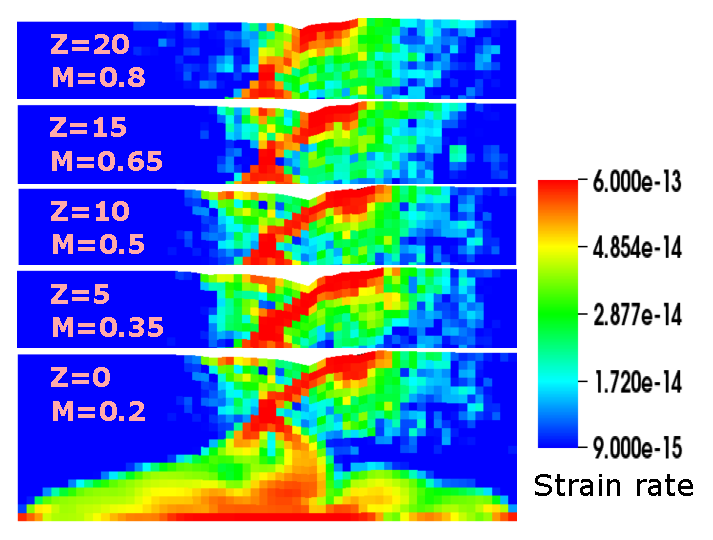
\includegraphics[width=0.6\textwidth]{fig_Results1_2.eps}
  \caption{M28LinT1 (Table~\hyperref[Tab1_1]{\ref{Tab1_1}}). Strain rate at 107.5kyr with five slices along ridge axis(Z axis).}
 \label{fig_Results1_2}
\end{figure}   

\begin{figure}[h]
  \centering
    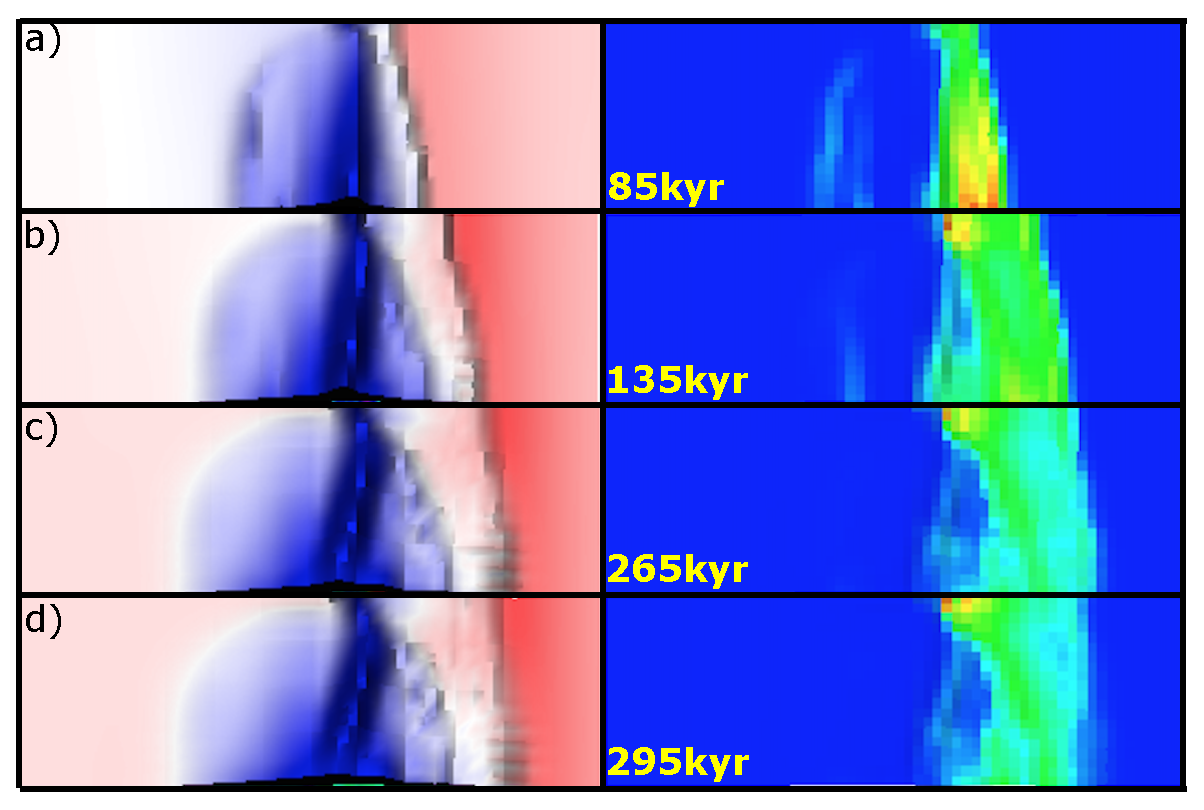
\includegraphics[width=0.6\textwidth]{fig_Results1_4.eps}
  \caption{M28LinT1 (Table~\hyperref[Tab1_1]{\ref{Tab1_1}}). Breakaway evolution through time. Viewing from top. Left column is topography at different time; Right column is plastic strain. They both share same color scales in the figure~\hyperref[fig_Results1_1]{\ref{fig_Results1_1}}. The offset between breakways along the ridge-axis in X-axis direction remains three elements until time 295kyr. It also shows that the lowest topography points along the ridge-axis start as a straigt line parellel with ridge-axis in a) and then gradually become oblique to the ridge-axis. Please see text for detail description.}
 \label{fig_Results1_4}
\end{figure}

At 240kyr (Figure~\hyperref[fig_Results1_1]{\ref{fig_Results1_1}.c}), the median valley further deepens and widens. The detachment keeps active and extends to $\sim$18km in length horizontally (longest at M$=0.2$) with the dip angle decreases from initially $\sim$60$\degree$ to 30$\degree$(at the root of the fault) and 0$\degree$ where the fault interface is exposed to the seafloor. However, for the detachment at the higher M side (especially the last three elements along the Z-axis), the dip angle remains high. The maximum relief between highest point in breakaway and lowest point in the median valley becomes larger than 1km. Corrugations show up at the lower M side, at the front tip of the extending fault interface. The lowest topography points inside the median valley evolves from a straight line parallel to the ridge-axis (Figure~\hyperref[fig_Results1_4]{\ref{fig_Results1_4}.a}) to a line oblique to the ridge-axis (Figure~\hyperref[fig_Results1_4]{\ref{fig_Results1_4}.b,c,d}). Initially, the lowest topography points are at the terminations of the detachment fault. Due to the coupling along the ridge-axis, fault propagates from front to back in a straight line parallel to the ridge-axis. However, as the dip angle of the detachment at the low M side begin to decrease due to bending of the crust at the footwall, along with excessive tensional stress results from low magma supply, the lowest topography point at the lower M side is pulled to the conjugate plate. While the lowest topography points at the high M side (M$>0.5$) are pushed away from the dike. Note that the oblique lowest topography points form not a straight line, but a curve that the lowest point remains near the ridge-axis at the high M side. This is due to the bending rate of the detachment at high M side is very low and thus the termination can remains near the ridge-axis.      
%{Important tecnique from discussion on Mar. 9th with Eunseo: 1. One way to analyze models is to make hypothesis to describe model behaviors and than use models to approve or reject it. If rejected, find a new hypothesis and do the same thing again.}
%\add[XT]{4. An new thinking on little termination or dip angle variation when M$<0.5$ as observed in %figure~\ref{fig_Results1_2}: why along-z hanging wall has little variation is because we have along z coupling, the rotational shear failure between along-z neighbors are so hard. and also, the more extension in M0.2 end is accommodated elastically by the whole plate to the left of the detachment fault which can be observed as lower topo(topography variation along ridge axis).} 

\add[XT]{One question needs to be answered: at 410 timesteps (205kyr), the breakaway at the front already extends 15km. If assumming a constant extending rate, it means a velocity of around 75km/Myr, much faster than half spreading rate 25km/Myr. If it is true, I need to change previous discussion on how fast breakaway being pulled away from ridge-axis.}

At 650kyr (Figure~\hyperref[fig_Results1_1]{\ref{fig_Results1_1}.d}), the median valley continues to deepen and widen. The breakaways along the ridge-axis already \annote[XT]{moved out of the model domain}{it should not, if breakaway move with 25km/yr(half spreading rate), since the distance between initial break (5km away from ridge center) and right wall of the model domain is about 25km which needs 1Myr to reach. But now is only 650kyr. Why is it?}. The fault offset is already larger than the thickness of the crust and the upper mantle materials begin to be exhumed to the surface. The previous fault interface bend over to a negative dip angle (dip in an opposite direction) and produces a dome shape OCC with corrugations on its surface parallel to the spreading direction. The previous lowest topography points evolve to a curve with bigger curvature. Compared to the inset in Figure~\hyperref[fig_Results1_1]{\ref{fig_Results1_1}.b}, the total length of the bending crust decreases. A hint of a near-axis secondary fault begin to initial at the high M side ($10<$Z$<15$) as a form of tension failure. \add[XT]{Its formation will be discussed in Discussion section accompanied by the stress status analysis. }

At 790kyr (Figure~\hyperref[fig_Results1_1]{\ref{fig_Results1_1}.e}), the initial tension failure immediately ajacent to the ridge center (hint of the secondary fault) begin to evolve and propagate to higher Z region.  

At 880kyr (Figure~\hyperref[fig_Results1_1]{\ref{fig_Results1_1}.f}), at the higher M side, the initial tension failure evolves to a high angle near-axis secondary normal fault and replace the initial detachment as indicated in the inset of transparent view of plastic strain.

At 910kyr (Figure~\hyperref[fig_Results1_1]{\ref{fig_Results1_1}.g}), the secondary normal fault results in a strong constrast in moving directions between high M side and low M side near the ridge-axis that at the high M side, previous hanging wall becomes footwall and moves with spreading direction on the right, however, at the low M side, due to deficit in magma supply, the hanging wall is coupled with conjugate plate and moves to the left as shown in the inset. This opposite direction motion creates a strong shear stress region $\sim$45$\degree$ oblique to the ridge-axis (inset of Figure~\hyperref[fig_Results1_1]{\ref{fig_Results1_1}.h}) and produces new lowest topography points align with it. Combined with previous lowest topography points, an ``X'' shape topography low is created.

Corrugations are observed in the model since 240kyr. It will be further discussed in the discussion chapter. There are two contributing factors, for one, trans-extenstional stresses are created due to offset of the breakaway as well as the variation in fault displacements along the ridge axis; for the other, the variation of the positions of the terminations of the detachment faults along the ridge-axis creates anastomosing faults that is mentioned in \citep{Smith2014}. This anastomosing faulting behavior is largely responsible for corrugations in our models.      

\subsubsection{Constant M along the ridge-axis }
\add[XT]{This section needs to be revised and add more details into the model description.}
Another reference model is the model with constant M$=0.8$ along the ridge axis as a comparison to the changing M models.

As shown in Figure~\hyperref[fig_Results1_3]{\ref{fig_Results1_3}}, this constant M along the ridge-axis model creates a median valley of $\sim 20km$ in width and $1\sim2km$ in depth which is similar to generally observation of Mid-Atlantic Ridges. The width and depth of the median valley is almost constant along the ridge-axis. The variation along the ridge-axis in breakaway and termination as well as the existence of corrugation mentioned in reference model one are not observed. 

\begin{figure}[h]
  \centering
    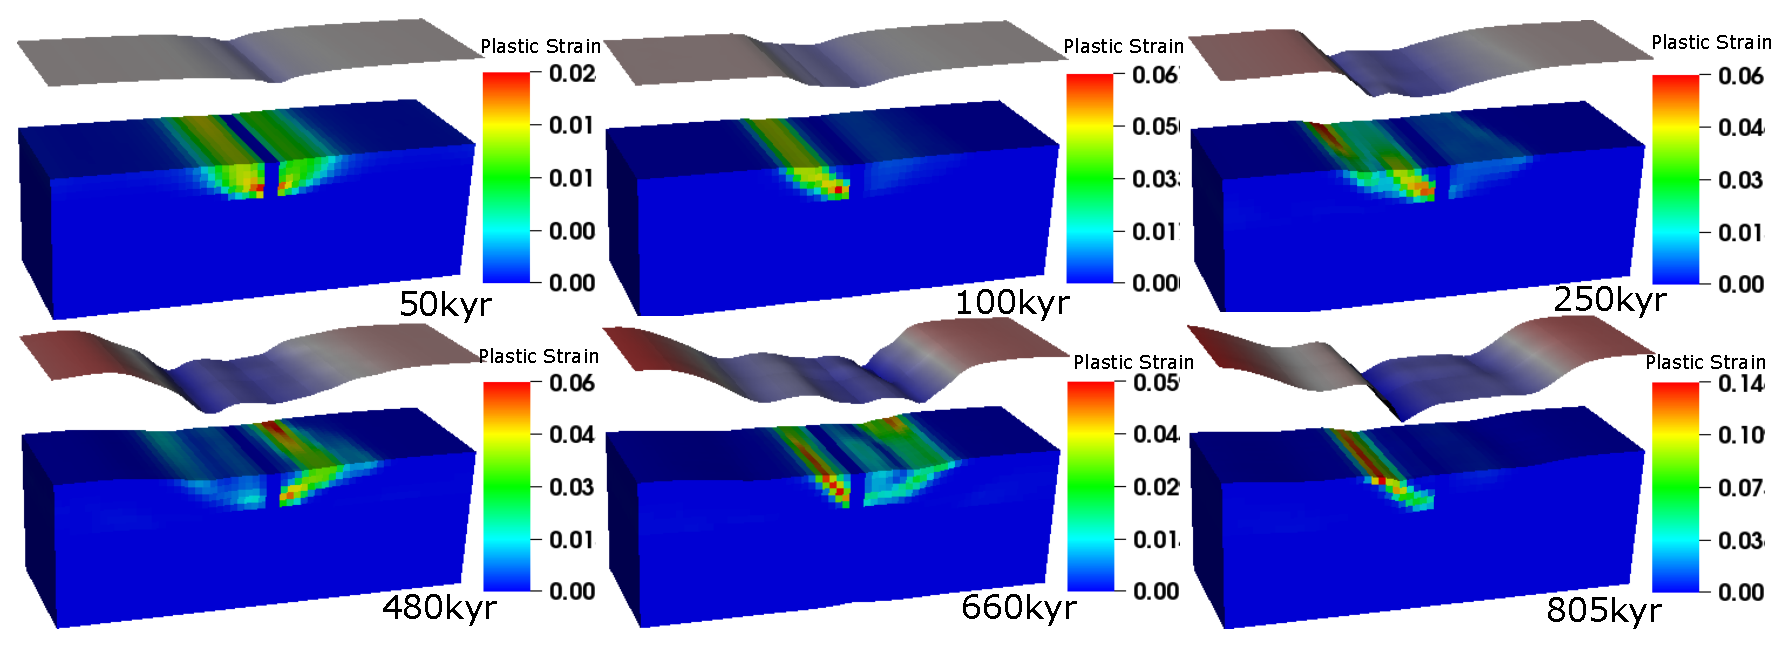
\includegraphics[width=1.0\textwidth]{fig_Results1_3.eps}
  \caption{M88ConT2 (Table~\hyperref[Tab1_1]{\ref{Tab1_1}}). Reference model two: constant M$=0.8$ along the ridge-axis (i.e. Z axis). Type two weakening.}
 \label{fig_Results1_3}
\end{figure}   

Based on the previous experience in pseudo-2D models or \citep{Lavier2000}, with higher characteristic fault offset ($\Delta X_{c}$) for Type two weakening compared with Type one weakening, the frequency of normal faulting alternation is higher for M$>0.5$ cases. However, interesting enough, when comparing pseudo-2D and 3D models when they are using Type two weakening under case of M$=0.8$, even though the 3D Model has a larger $\Delta X_{c}$ of 1km than that of pseudo-2D model of 0.5kmr, 3D model has a lower frequency of faulting alternation. Since M is constant 0.8 along the ridge-axis, the effect of along ridge couplingthat resists alternation need not be considered. One possibility is that the resisting bending force increase in a higher rate than linear with respect to increasing the length of the ridge segment (Z$_{max}$ km).  

\subsection{Tables of all the data points}

Currently, we have run \annote[XT]{hundreds of}{find out exactly number that will be used in 2D model results conclusion} Psedudo-2D models for initial setup and benchmarking with previous studies (e.g. \citep{Buck2005} and \citep{Tucholke2008}). Based on those Pseudo-2D models, we further ran 11$+$1 (11 models with M variation along the ridge-axis and 1 model with constant M$=0.8$ along the ridge-axis) 3D models shown in Table~\hyperref[Tab1_1]{\ref{Tab1_1}}. The available data points are limited due to the huge computation expenses for 3D models (For each model to be run to 2Myr, usually needs 192 cores for about 2 days (around 10000 SUs). \add[XT]{use 96 cores can improve the efficiency a little bit (Longer time but smaller amount of SUs needed).})

\begin{table}[h]
\centering
\begin{tabular}{l l l l l}
\hline
\hline
Model& M range & Functional Form & Type of weakening & For short \\ 
\hline
1    &  M28    &   Linear        & Type one   &  M28LinT1\\
\hline
2    &  M28    &   Sinusoidal    & Type one   &  M28SinT1\\
\hline
3    &  M28    &   Square Root   & Type one   &  M28SqrtT1 \\
\hline
4    &  M57    &   Linear        & Type one   &  M57LinT1 \\
\hline
5    &  M57    &   Sinusoidal    & Type one   &  M57SinT1 \\
\hline
6    &  M57    &   Sinusoidal    & Type two   &  M57SinT2 \\
\hline
7    &  M57    &   Square Root   & Type two   &  M57SqrtT2  \\
\hline
8    &  M58    &   Sinusoidal    & Type one   &  M58SinT1  \\
\hline
9    &  M58    &   Sinusoidal    & Type two   &  M58SinT2   \\
\hline
10   &  M58    &   Square Root   & Type one   &  M58SqrtT1   \\
\hline
11   &  M58    &   Square Root   & Type two   &  M58SqrtT2   \\
\hline
12   &  M88    &   Constant      & Type two   &  M88ConT2 \\

\hline
\hline
\end{tabular}

\caption{List of 3D numerical experiments}
\label{Tab1_1}
\end{table}

\begin{table}[hc]
\begin{small}
\begin{center}
\begin{tabular}{||l|l||l|l||l|l||}
\hline
A & Alternating Fault & C & Corrugation & SL & Shear Topography Low \\
\hline
NA& Not Alternating & SF & Secondary Fault on one side & CB & Cut Back   \\
\hline
DD &  Double Dome  & AM    & Atlantis Massif &  &   \\
\hline
\end{tabular}
\end{center}
\end{small}
\caption{Model behaviors in short.}
\label{Tab1}
\end{table}

Based on the 11 models with M variation, we observed eight first-order behaviors as shown in Table~\hyperref[Tab1]{\ref{Tab1}}. 

\begin{table}[h]
\begin{small}
\begin{center}
\begin{tabular}{|l|p{3.5cm}|p{3.5cm}|p{3.5cm}|}
\hline
\diagbox[width=6em]{Type}{M range}&
M28&M57&M58\\
\hline
Type one &NA; C; SL; SF$_{1500kyr}$; DD    &NA; C; SF$_{1380kyr}$; CB$_{330kyr}$; AM(opposite z)     &    \\
\hline
Type two &    &     &    \\
\hline
\end{tabular}
\end{center}
\end{small}
\caption{Linear functional form.}
\end{table}

\begin{center}
\begin{table}[h!]
\begin{small}
\begin{tabular}{|l|p{3.5cm}|p{3.5cm}|p{3.5cm}|}
\hline
\diagbox[width=6em]{Type}{M range}&
M28&M57&M58\\
\hline
Type one & NA; C; SL; SF$_{995kyr}$ & NA; C; SL; SF$_{760kyr;1320kyr}$; CB$_{520kyr}$; AM & NA; C; SL; CB$_{510kyr}$; SF$_{760kyr;1140kyr;1990kyr}$   \\
\hline
Type two &    &NA; C; SL; SF$_{680kyr}$; CB$_{905kyr}$     & A$_{450kyr;600kyr}$; C(only at low M); CB$_{990kyr}$   \\
\hline
\end{tabular}
\end{small}
\caption{Sinusoidal functional form.}
\end{table}
\end{center}

\begin{table}[h!]
\begin{small}
\begin{center}
\begin{tabular}{|l|p{3.5cm}|p{3.5cm}|p{3.5cm}|}
\hline
\diagbox[width=6em]{Type}{M range}&
M28&M57&M58\\
\hline
Type one & NA; C; SL; CB$_{205kyr;330kyr;1025kyr}$   &      & NA; C$_{1770kyr}$(due to shear with dif wave length); SF$_{860kyr}$(high M); SF$_{1190kyr}$(low M)(Dog Bone); SF$_{1690kyr}$    \\
\hline
Type two &    & NA; C; SF$_{435kyr;1060kyr}$; CB$_{585kyr}$; CB$_{735kyr}$; CB$_{910kyr}$; CB$_{970kyr}$    & A$_{550kyr;920kyr}$; C; CB$_{400kyr}$    \\
\hline
\end{tabular}
\end{center}
\end{small}
\caption{Square root functional form.}
\end{table}

Based on the available data points as shown in the tables, we are able to compare the model results with respect to three factors: 1) Variation of the range of M; 2) Variation of the functional form and 3) Influence of weakening rate. 

\subsection{Variation of the functional form}
How magma supply varies along the MORs ridge-axis remains a current research question and we do not have direct quantitative observation over it. However, from indirect geophysical studies (e.g. gravity, seismology), people suggest a general qualitative pattern of 20 to 50 km long second-order ridge segment with magma mostly supply at the segment center and decreases to the end \citep{Carbotte2015}. Since we do not know exatly how magma supply varies along the ridge, we try three functional forms (linear, sinusoidal and square root) for its variation along the ridge-axis.

\subsubsection{Comparing M28 in terms of linear, sinusoidal and square root}
As shown in the tables, M28 with Type one weakening is the only M range that has three functional forms data points available. There are two phenomena that show distinct differences with respect to different functional forms. One is the geometry and timing of the secondary fault. The other is the ``Cut back'' behavior mostly observed in the square root model.

\begin{figure}[h]
  \centering
    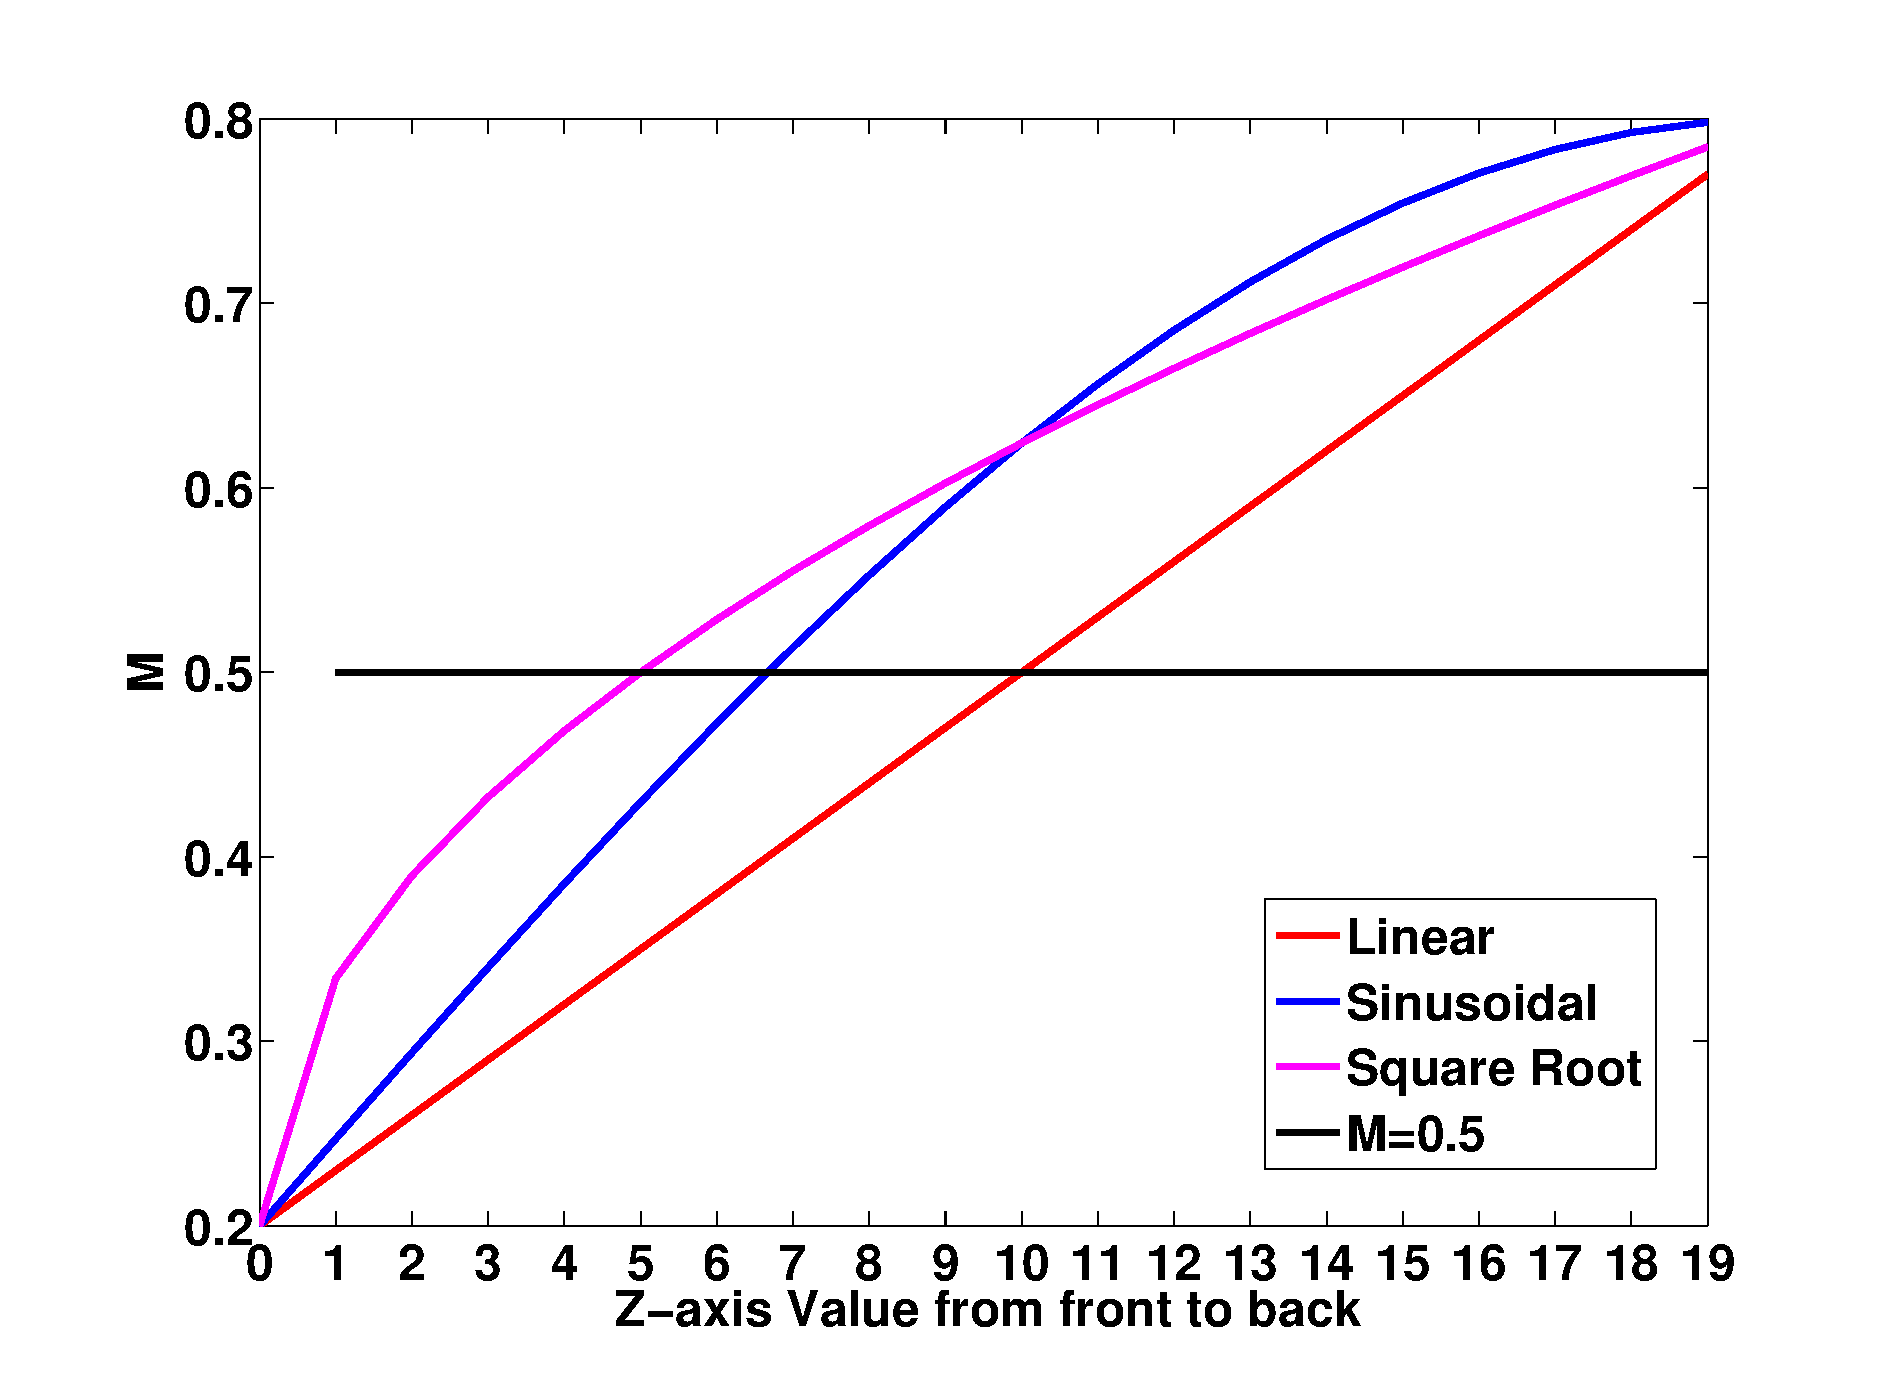
\includegraphics[width=0.6\textwidth]{fig_Results3_1.eps}
  \caption{Three functional forms of M variation comparison. They begin to exceed the M$=0.5$ black line at Z=10, 7, 5 for linear, sinusoidal and square root respectively.}
 \label{fig_Results3_1}
\end{figure}   

\paragraph{Secondary Fault}

For linear, the secondary fault at higher M side begins to take place at around 900kyrs (Figure~\hyperref[fig_Results4_2]{\ref{fig_Results4_2}}), its spatial distribution is at M$>0.5$ region. It nucleates from the shear low (ridge center where M$=0.5$) to the M$=0.8$ end (Figure~\hyperref[fig_Results3_1]{\ref{fig_Results3_1}} where the red line begin to exceeds 0.5 at Z$=10$). As it evolve, the initial detachment becomes inactive. This secondary fault creates another dome with initial composition likely to be volcanic rather than ultramafic, however, as it evolves, if it can last long enough to cut through the whole crust, mantle materials might exhume to the surface. The composition of the domes observed at Kane magamullions is similar to this mechanism between ultramafic babel dome and eastern to it the crustal inside-corner high. 

\begin{figure}[h]
  \centering
    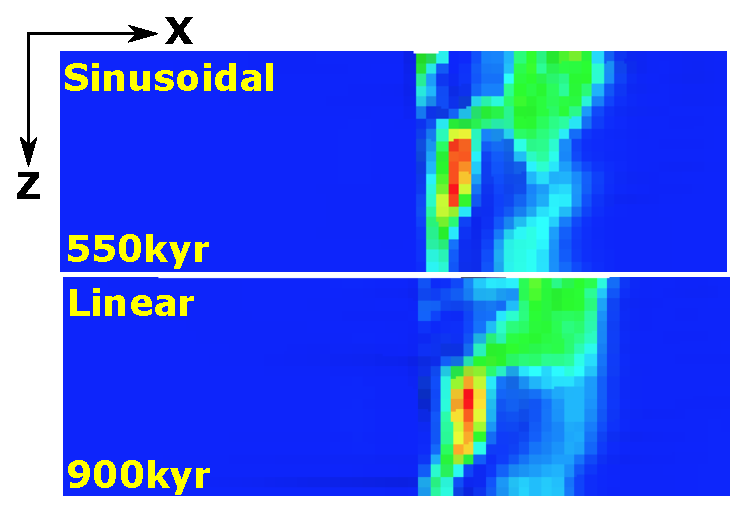
\includegraphics[width=0.6\textwidth]{fig_Results4_2_secondary_fault_length_comparison.eps}
  \caption{M28LinT1 versus M28SinT1 (Table~\hyperref[Tab1_1]{\ref{Tab1_1}}). Secondary fault length comparison between linear and sinusoidal. Around 13 elements in length for sinusoidal compared to 11 elements for linear.}
 \label{fig_Results4_2}
\end{figure}   

For sinusoidal, the secondary fault begins to form at a much earlier time around 550kyrs (Figure~\hyperref[fig_Results4_2]{\ref{fig_Results4_2}}), this is due to the total area of M$>0.5$ for sinusoidal functional form is higher than that of linear. Qualitatively, the total force to push the hanging wall of the detachment away from the dike for sinusoidal is larger than that of linear. The larger the force, the faster the detachment moves off axis, the earlier the secondary fault will appear. In addition, the total length of the secondary fault is longer due to the total length of M that is above 0.5 is bigger than that of the linear model (Figure~\hyperref[fig_Results3_1]{\ref{fig_Results3_1}}). 
For square root, there is no secondary fault forming because the ``cut back'' behavior releases the tensional stress in the hanging wall.

\paragraph{Cut back}

\begin{figure}[h]
  \centering
    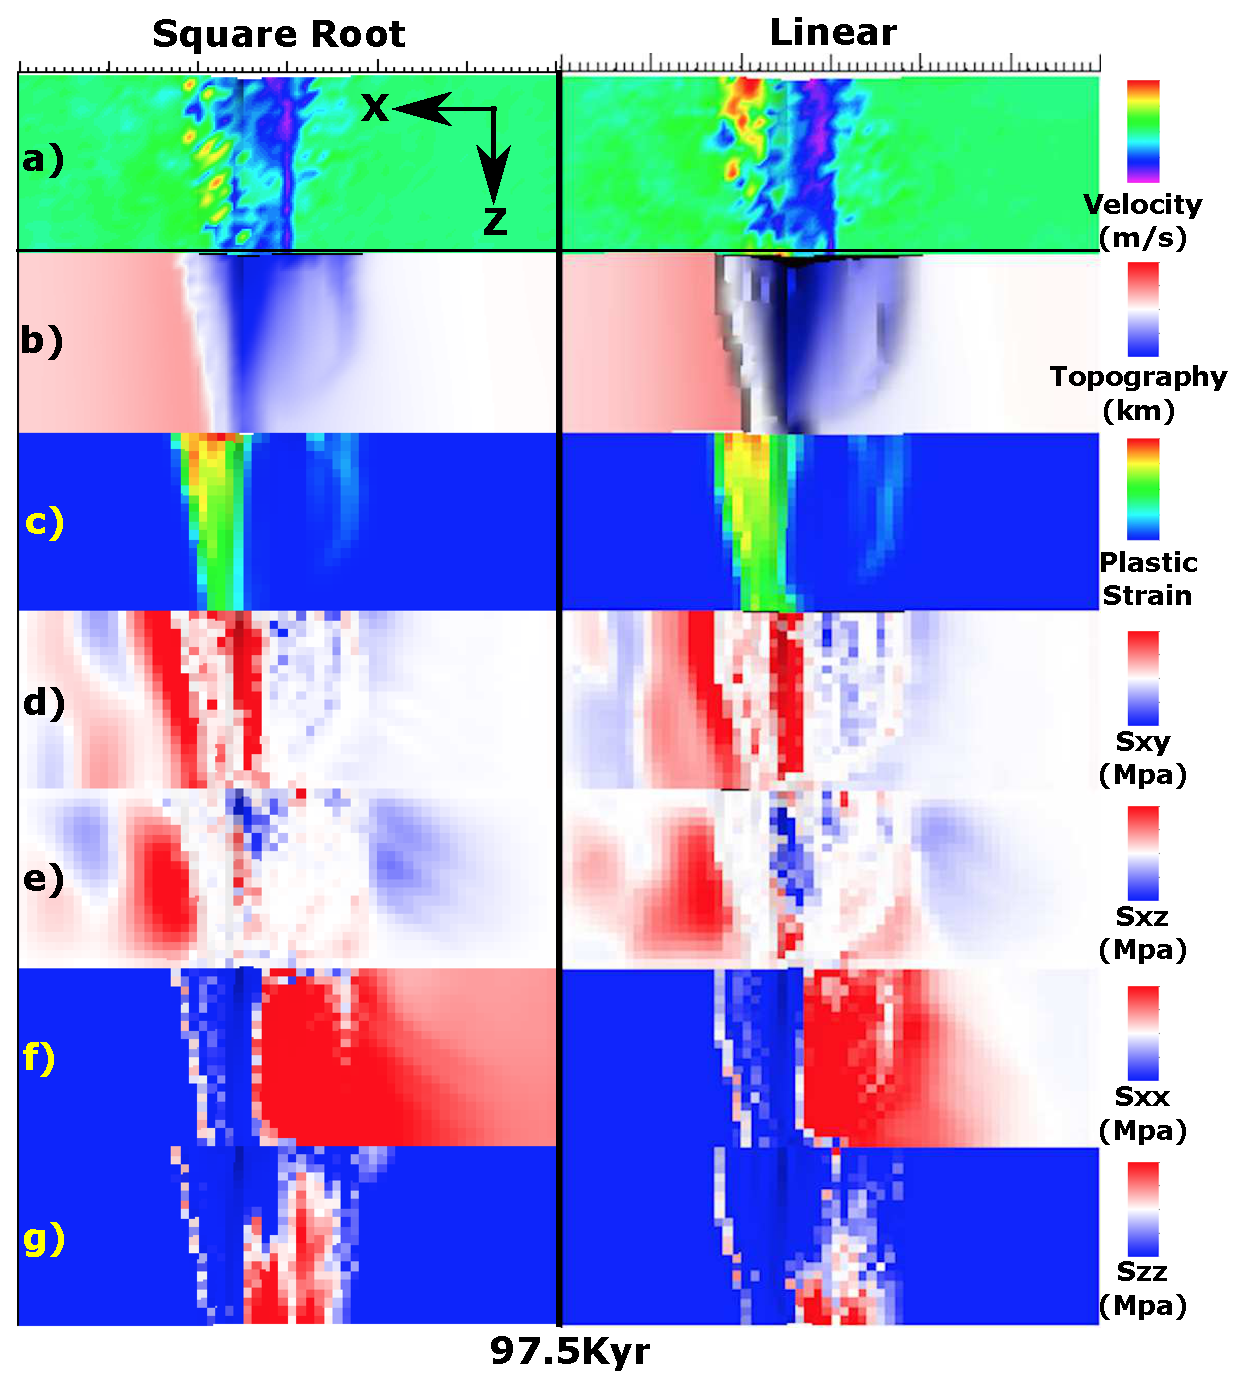
\includegraphics[width=0.6\textwidth]{fig_Results4_3_sqrt_vs_lin_cut_back_97kyr.eps}
  \caption{M28LinT1 versus M28SqrtT1 (Table~\hyperref[Tab1_1]{\ref{Tab1_1}}) at 97kyr. View from top of the model.}
 \label{fig_Results4_3_1}
\end{figure}  

\begin{figure}[h]
  \centering
    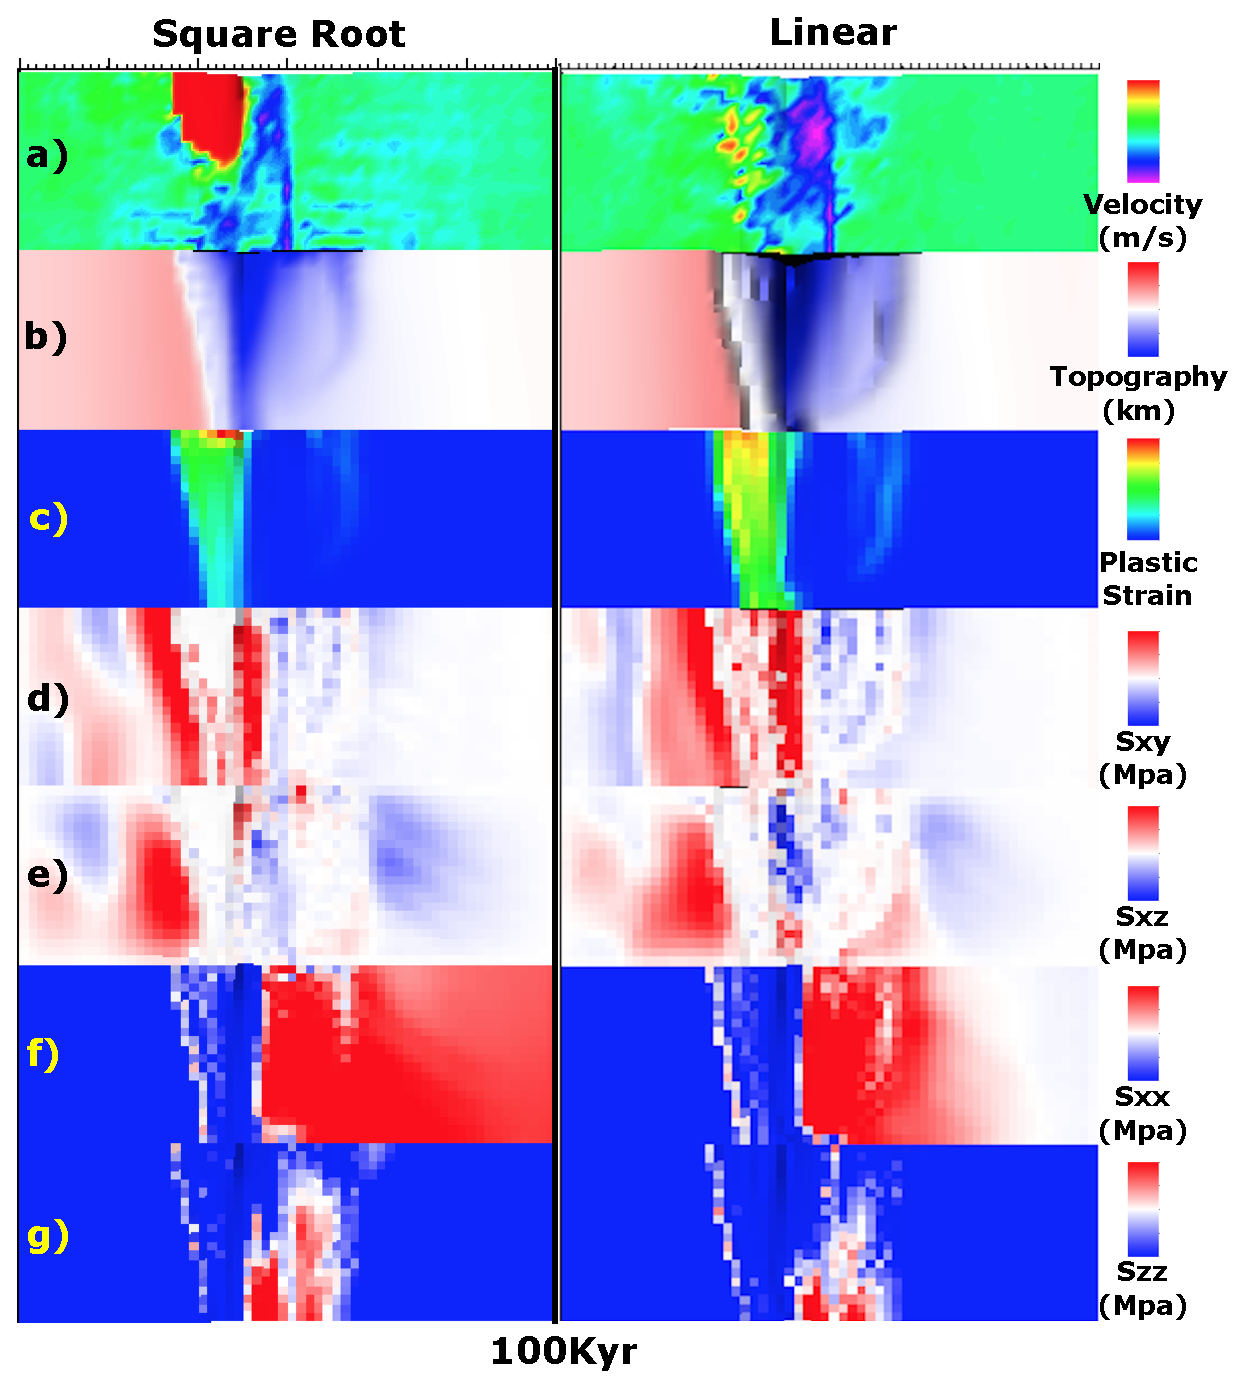
\includegraphics[width=0.6\textwidth]{fig_Results4_3_sqrt_vs_lin_cut_back_100kyr.eps}
  \caption{M28LinT1 versus M28SqrtT1 (Table~\hyperref[Tab1_1]{\ref{Tab1_1}}) at 100kyr. View from top of the model.}
 \label{fig_Results4_3_2}
\end{figure} 

\begin{figure}[h]
  \centering
    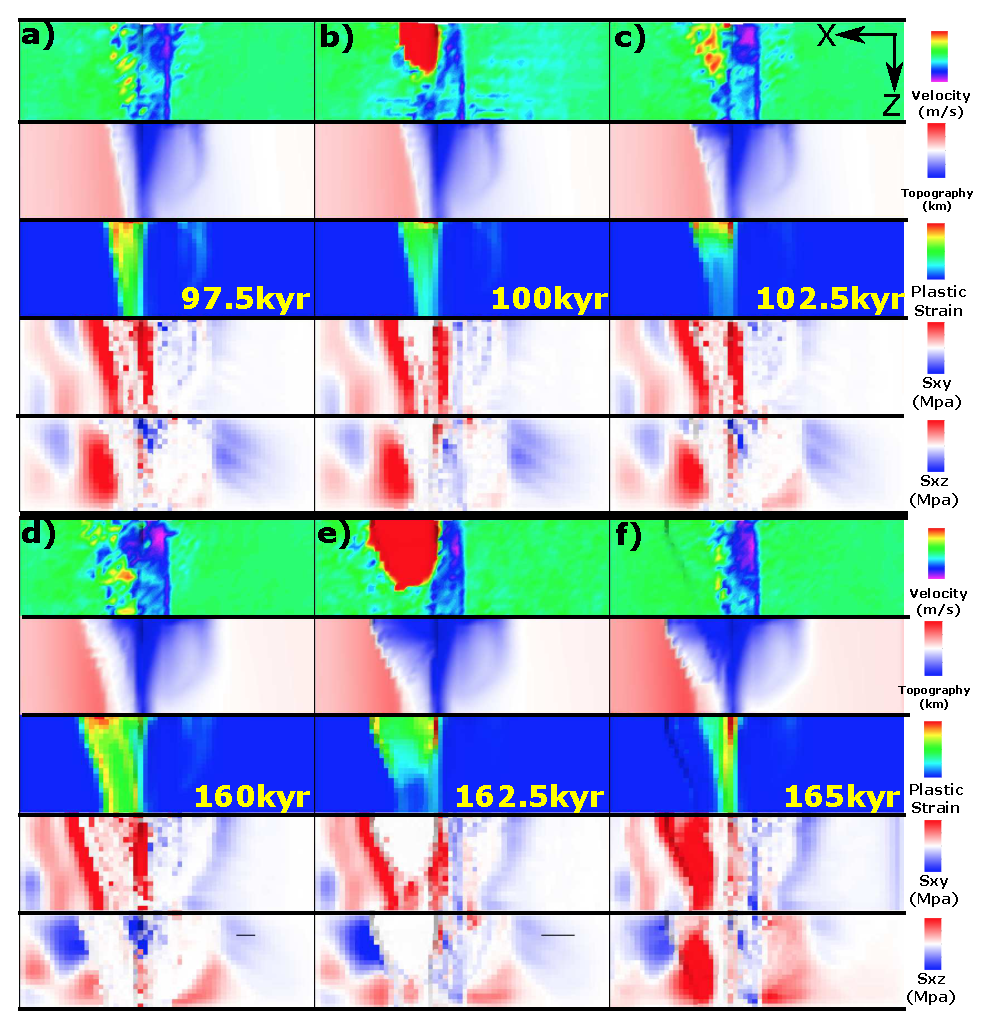
\includegraphics[width=0.8\textwidth]{fig_Results4_4_sqrt_cut_back_with_time.eps}
  \caption{M28SqrtT1 (Table~\hyperref[Tab1_1]{\ref{Tab1_1}}). Cut back behaviors in square root functional form model with different time.}
 \label{fig_Results4_4}
\end{figure}   

\begin{figure}[h]
  \centering
    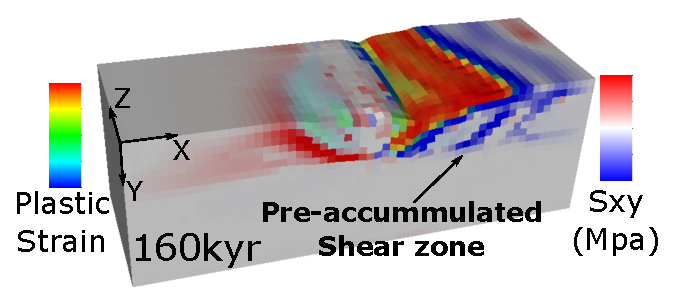
\includegraphics[width=0.6\textwidth]{fig_Results4_5_sqrt_cut_back_pre_accummulated_shear_zone.eps}
  \caption{M28SqrtT1 (Table~\hyperref[Tab1_1]{\ref{Tab1_1}}). Square root functional form model at 160kyr. Pre-accummulated shear zone increase the shear force and cut the weak detachment front tip}
 \label{fig_Results4_5}
\end{figure}   

The cut back happens mostly in the square root model. Since the linear model and the square root model have more obvious difference in terms of the cut back behavior, here, we only compare linear and square root. There are several factors contribute to the cut back behavior. First, at the higher M side, the amount of diking for the square root model is ubiquitously larger than that of the linear one (Figure~\hyperref[fig_Results3_1]{\ref{fig_Results3_1}}). This leads to a slower bending detachment at the high M side for the square root model. Second, the totoal length of the ridge segment with M$>0.5$ for the square root model is also longer than that of the linear one (Figure~\hyperref[fig_Results3_1]{\ref{fig_Results3_1}}). This results in that at the low M side, $\sigma_{xz}$ is focused at low Z ajacent to the ridge-axis (Figure~\hyperref[fig_Results4_3_1]{\ref{fig_Results4_3_1}.e}), however for linear is spread out to Z higher than 10. Third, due to higher value of $\frac{dM}{dZ}$ for square root when Z$<5$, the along ridge-axis shear $\sigma_{xz}$ for square root will be accummulating faster, which produces larger strike-slip force to cut the hanging wall at the low M side. Fourth, as observed in the model (Figure~\hyperref[fig_Results4_3_1]{\ref{fig_Results4_3_1}.c}), the parallel to spreading direction offset between breakaways along the ridge-axis is 4km for the square root model compared to 3km for the linear model. This causes the square root model to experience bigger shear stress $\sigma_{xy}$ both immediately beneath and above the fault interface at the low M side (Figure~\hyperref[fig_Results4_3_1]{\ref{fig_Results4_3_1}.d}). Fifth, as shown in Figure~\hyperref[fig_Results4_8]{\ref{fig_Results4_8}}, due to bending of the crust at the footwall side, below the blue neutral plane, $\sigma_{xx}>0$, meaning tensional stress being accummulated as fault develops. The resulting force tends to unbend the bended crust and drag down the connecting surface (the future decoupled hanging wall). All five factors together assist in the decouple of the hanging wall at the low M side as described in detail in the next paragraph.

\begin{figure}[h]
  \centering
    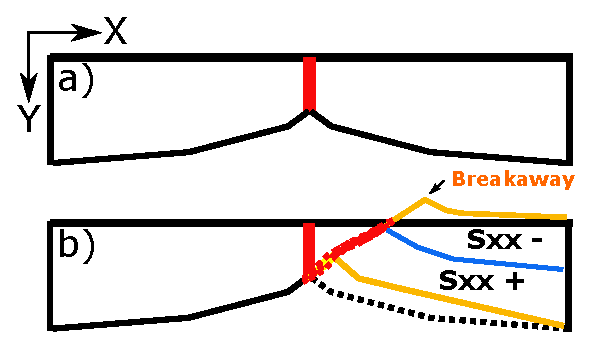
\includegraphics[width=0.6\textwidth]{fig_Results4_8_sqrt_cut_back_bending_cartoon.eps}
  \caption{Bending stress illustration. The blue line is the neutral plane where $\sigma_{xx}=0$. Above the neutral plane is compression and beneath it is tension. Due to sea water pressure and lithostatic pressure, compression is generally one degree magnitude larger than tension.}
 \label{fig_Results4_8}
\end{figure}

\begin{figure}[h]
  \centering
    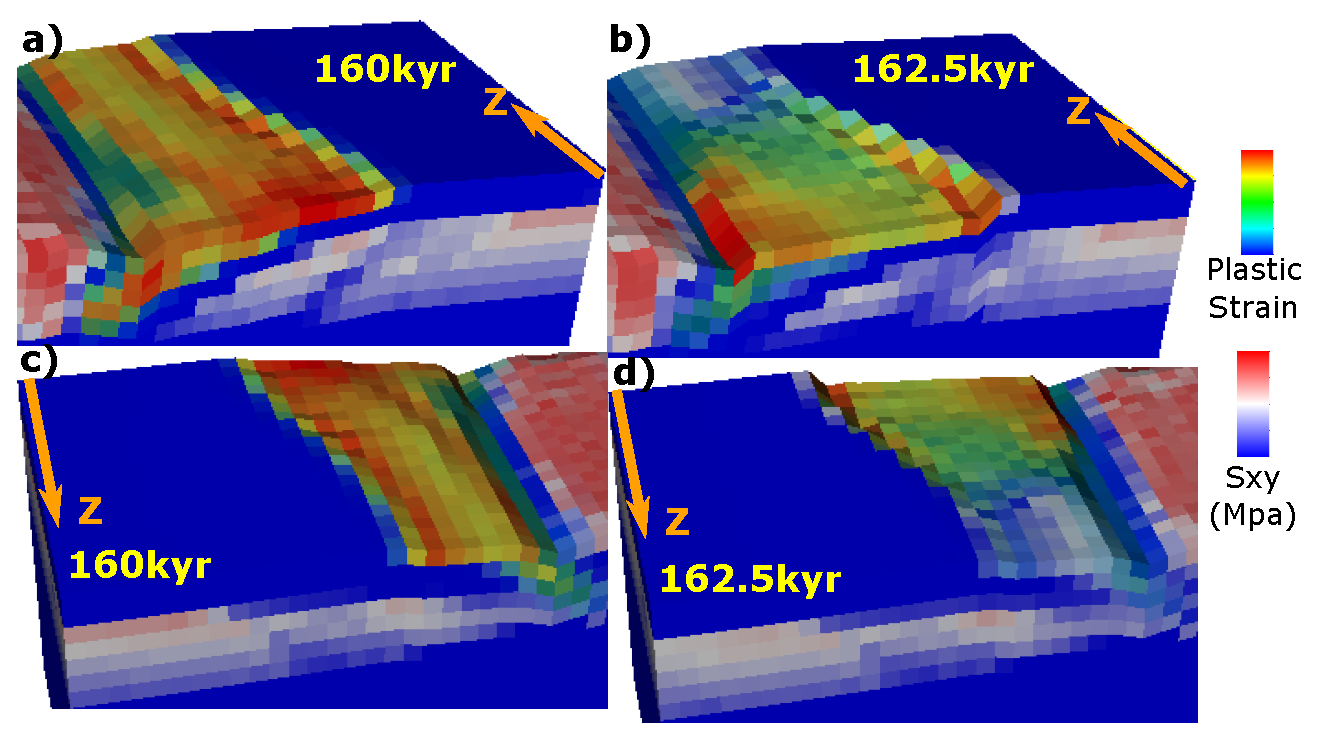
\includegraphics[width=0.6\textwidth]{fig_Results4_6_sqrt_cut_back_bending_drop.eps}
  \caption{M28SqrtT1 (Table~\hyperref[Tab1_1]{\ref{Tab1_1}}). Bending stress drop in the crust close to dike due to cut back behavior.}
 \label{fig_Results4_6}
\end{figure}

%(Figure~\hyperref[fig_Results4_6]{\ref{fig_Results4_6}})reveals that
In the Figure~\hyperref[fig_Results4_4]{\ref{fig_Results4_4}}, the hanging wall rebounds backwards to the dike in a high velocity (Figure~\hyperref[fig_Results4_4]{\ref{fig_Results4_4}.b,e (velocity)}) accompanied with a sudden topography drop (Figure~\hyperref[fig_Results4_4]{\ref{fig_Results4_4}.b) compared to c); d) compared to e) (in the second row)}). This behavior is triggered when the front tip of the weak detachment extends further away from the ridge-axis and reaches a pre-accummulated shear zone (Figure~\hyperref[fig_Results4_5]{\ref{fig_Results4_5}}). The pre-accummulated shear zone adds extra shear force to the weak (Figure~\hyperref[fig_Results4_4]{\ref{fig_Results4_4}}.d(third row: plastic strain)) as well as shear stresses accummulated (Figure~\hyperref[fig_Results4_4]{\ref{fig_Results4_4}.d}(fourth and fifth row: $\sigma_{xy}$ and $\sigma_{xz}$)) fault interface and together with the five factors mentioned in the previous paragraph result in the cut back behavior. The cut back produces a continuous high angle fault scarp with a relief of $\sim 1km$ aligns to the initial breakaway and extends for about 20 kilometer in length (Figure~\hyperref[fig_Results4_4]{\ref{fig_Results4_4}.e (second row: topography)}). Its distance to the ridge-axis varies along the Z-axis and this result can be used to indicate the magma supply variation in the nature as will be discussed in the ``Discussion'' chapter. \add[XT]{To be discussed. as a reminder}

During the cut back process, the tensional bending stress are released at the low M side ($0<$Z$<7$) in the left tip of the bended crust (Figure~\hyperref[fig_Results4_6]{\ref{fig_Results4_6}.a compared to b}), however, in the higher M side, the tensional bending stress keeps accummulating due to the far field extension (Figure~\hyperref[fig_Results4_6]{\ref{fig_Results4_6}.c compared to d}). This behavior assists in the decouple between low M and high M side hanging walls. 

Once the cut back happens at 162.5kyr, the $\sigma_{xy}$, $\sigma_{xz}$ and $\sigma_{xx}$ are released (Figure~\hyperref[fig_Results4_4]{\ref{fig_Results4_4}.e (fourth and fifth row: $\sigma_{xy}$ and $\sigma_{xz}$)}). The plastic strain near the ridge-axis at low M side reaches a maximum of $\sim$0.9 (Figure~\hyperref[fig_Results4_4]{\ref{fig_Results4_4}.e (third row: plastic strain)}) compared to $\sim$0.3 before and after. This is due to the sudden backward motion squeezes the end element of the hanging wall near the ridge-axis and later be released by the continuous extension.

After the cut back, the termination of the detachment recedes backwards for about 7 kilometer towards the ridge-axis (Figure~\hyperref[fig_Results4_4]{\ref{fig_Results4_4}.f (third row: plastic strain)}) (termination fronts are always consistent with tension stresses in $\sigma_{xx}$ and $\sigma_{zz}$ as well as with plastic strain front(due to healing, high plastic strain region corresponds only to region with continuously deformation) (Figure~\hyperref[fig_Results4_3_1]{\ref{fig_Results4_3_1}} and Figure~\hyperref[fig_Results4_3_2]{\ref{fig_Results4_3_2}})). This behavior helps maintain a high angle normal fault. Different from the linear and sinusoidal models that the detachments at the low M side will rotate to a very low angle, square root model doesn't. In addition, $\sigma_{xy}$ and $\sigma_{xz}$ soon fill in the area between cut back created fault scarp and the new termination (Figure~\hyperref[fig_Results4_4]{\ref{fig_Results4_4}.f (fourth and fifth row: $\sigma_{xy}$ and $\sigma_{xz}$)} because $\sigma_{xy}$ always accummulates immediately beneath the normal fault interface and the red $\sigma_{xz}$ left to the new termination is due to the along ridge-axis variatioin in the rate of fault slip (low M side larger).  

\begin{figure}[h]
  \centering
    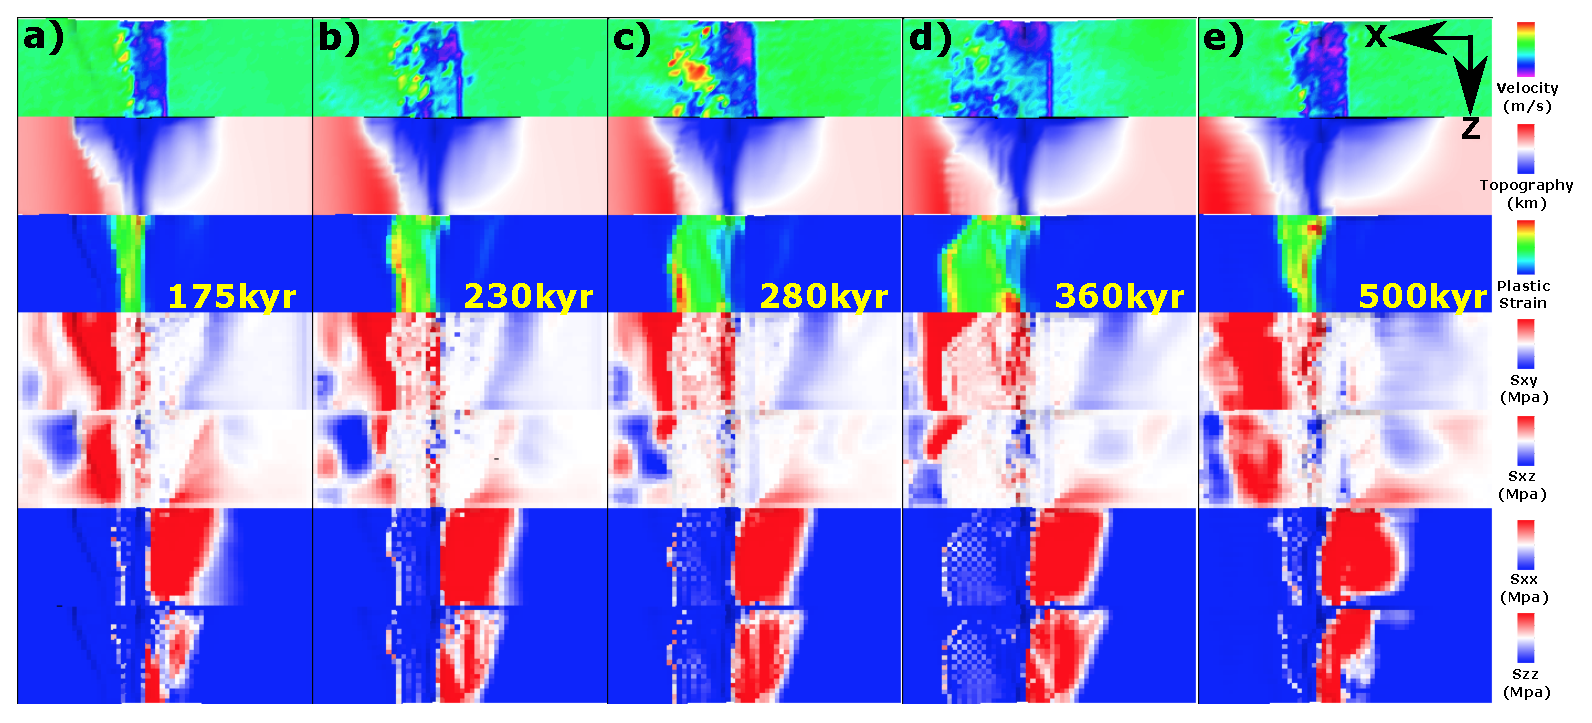
\includegraphics[width=1.0\textwidth]{fig_Results4_9_sqrt_cut_back_new_fault_chase.eps}
  \caption{M28SqrtT1 (Table~\hyperref[Tab1_1]{\ref{Tab1_1}}). New fault front chase after initial abandoned breakaway.}
 \label{fig_Results4_9}
\end{figure}

There is one phenomenon very interesting and counter-intuitive that worth describing here. After the cut back, and termination retreat, the evolution of the detachment fronts is opposite to initiall or to the general behavior in the linear and sinusoidal models. The termination front at the high M side extends faster and further after the cut back (Figure~\hyperref[fig_Results4_9]{\ref{fig_Results4_9}}). This is partly related to the unbending decouple phenomenon we described ealier that the tensional stress are released at the low M side but continues to accummulate in the high M side which results from the cut back unbending in the low M side. Since the tensional stress is released in the low M side, it needs time to accummulate to where it was and then start from there to drag the new near ridge-axis fault away from the ridge-axis while at the high M side the increasing tensional stress will directly lead to a fast extending fault front. Thus create the behavior. \add[XT]{One question is, how to explain that the fault front is moving much faster than the initial abandoned breakaway? New fault front soon reach the old breakaway.} This phenomenon is largely responsible for the corrugations observed. It create a ``X'' shape ``scan'' that first ``scan'' the topography with faster low M side (Figure~\hyperref[fig_Results4_4]{\ref{fig_Results4_4}.d and e}) and than with faster high M side (Figure~\hyperref[fig_Results4_9]{\ref{fig_Results4_9}.c and d}). This results in curved terminations with hundreds to several kilometers wavelengths that directly create parallel to spreading direction corrugations.    

\begin{figure}[h]
  \centering
    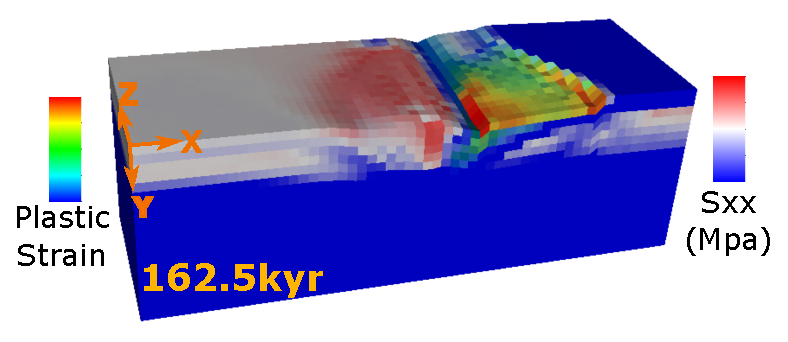
\includegraphics[width=0.6\textwidth]{fig_Results4_7_sqrt_cut_back_conjugate_Sxx.eps}
  \caption{M28SqrtT1 (Table~\hyperref[Tab1_1]{\ref{Tab1_1}}). Higher $\sigma_{xx}$ in the median valley of conjugate plate at low M side. }
 \label{fig_Results4_7}
\end{figure}

In addition, the higher $\sigma_{xx}$ in the median valley of conjugate plate at low M side (Figure~\hyperref[fig_Results4_7]{\ref{fig_Results4_7}}) is because the brittle crust is thinnest at the median valley, thus when same amount of force propagates from far field extension to the center median valley, the stress will increases.    

\subsection{Influence of weakening rate}

According to our available twelve 3D models, we have three pairs of models that both have Type one and Type two weakening while the range of M and functional form are maintained to be the same. They are M57(sinusoidal), M58(sinusoidal) and M58(square root). We will describe their differences respectively. 

\begin{figure}[h]
 \centering
  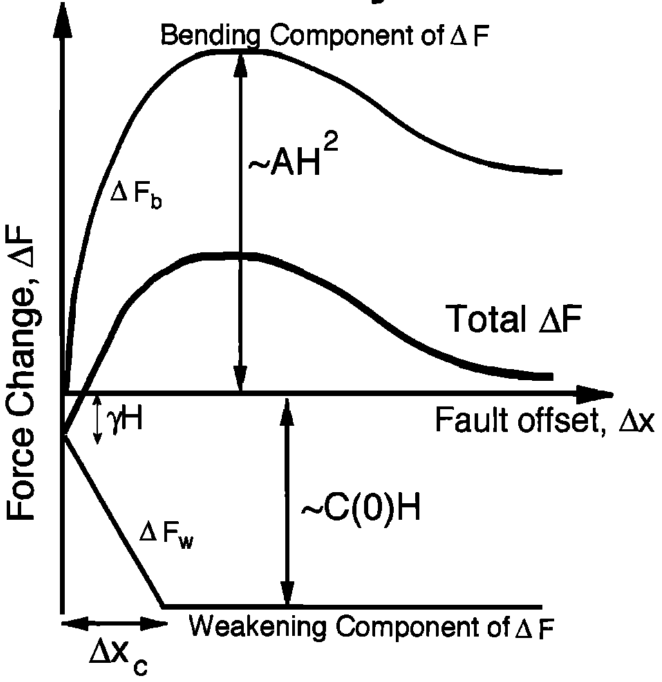
\includegraphics[width=0.45\textwidth]{fig_Results_Weakening_1_tradeOff_bend_weak.png}
 \caption{Trade-off between change in bending force $\Delta F_{b}$ and weakening in the fault interface $\Delta F_{w}$. H is the thickness of the brittle crust and $\gamma$ is the size of initial weak perturbation and A defines the maximum bending force change. (For more details, please refer to \citep{Lavier2000})}
 \label{fig_Results_Weakening_1}
\end{figure}

Before we move on to each of the pairs, the framework studied by \citep{Lavier2000} needs to be mentioned here for better understanding the model behaviors observed in our model results. There is a trade-off between change in bending force $\Delta F_{b}$ as a function of fault offset $\Delta X$ and force change $\Delta F_{w}$ as a function of  $\Delta X$ due to strain weakening. As described in \citep{Lavier2000}, higher characteristic fault offset ($\Delta X_{c}$) or slower strain weakening results in multiple faults rather than only one fault lasting. Whether conjugate fault and even multiple faults can be produced depends on the local stress condition. The strength weakening of the existed fault combines with how much bending force resists the fault to keep offseting play a major role in determining the stress state at the other areas. As the sea-floor keeps spreading and  $\Delta X$ increasing, the change in bending force $\Delta F_{b}$ increases and the strength at the fault interface decreases due to weakenging $\Delta F_{w}$ (Figure~\hyperref[fig_Results_Weakening_1]{\ref{fig_Results_Weakening_1}}). If the net force change $\Delta F = \Delta F_{b}+ \Delta F_{w}$ is positive, it means that it is getting harder and harder to maintain the existing fault and stress will begin to accummulate at the other areas which eventually break another fault. $\Delta F_{b}$ initially increases fast with respect to $\Delta X$ and then when the breakaway bends over, it reaches its peak value and begin to decreases a little and maintains at a constant value. If the strain weakenging is fast enough that the net effect force $\Delta F$ is always negative, then most of the stress will be released by the existing fault and thus no conjugate or multiple faults will be created. 

Our model results verify this analysis that only Type two weakening (slower weakening with higher $\Delta X_{c}$) can produce an alternating normal fault on the conjugate plate.

\subsubsection{M57 sinusoidal Type one versus M57 sinusoidal Type two}

There are very distinct differences between the two models. They share same functional form (sinusoidal) as well as M range (M57).

\begin{figure}[h]
 \centering
  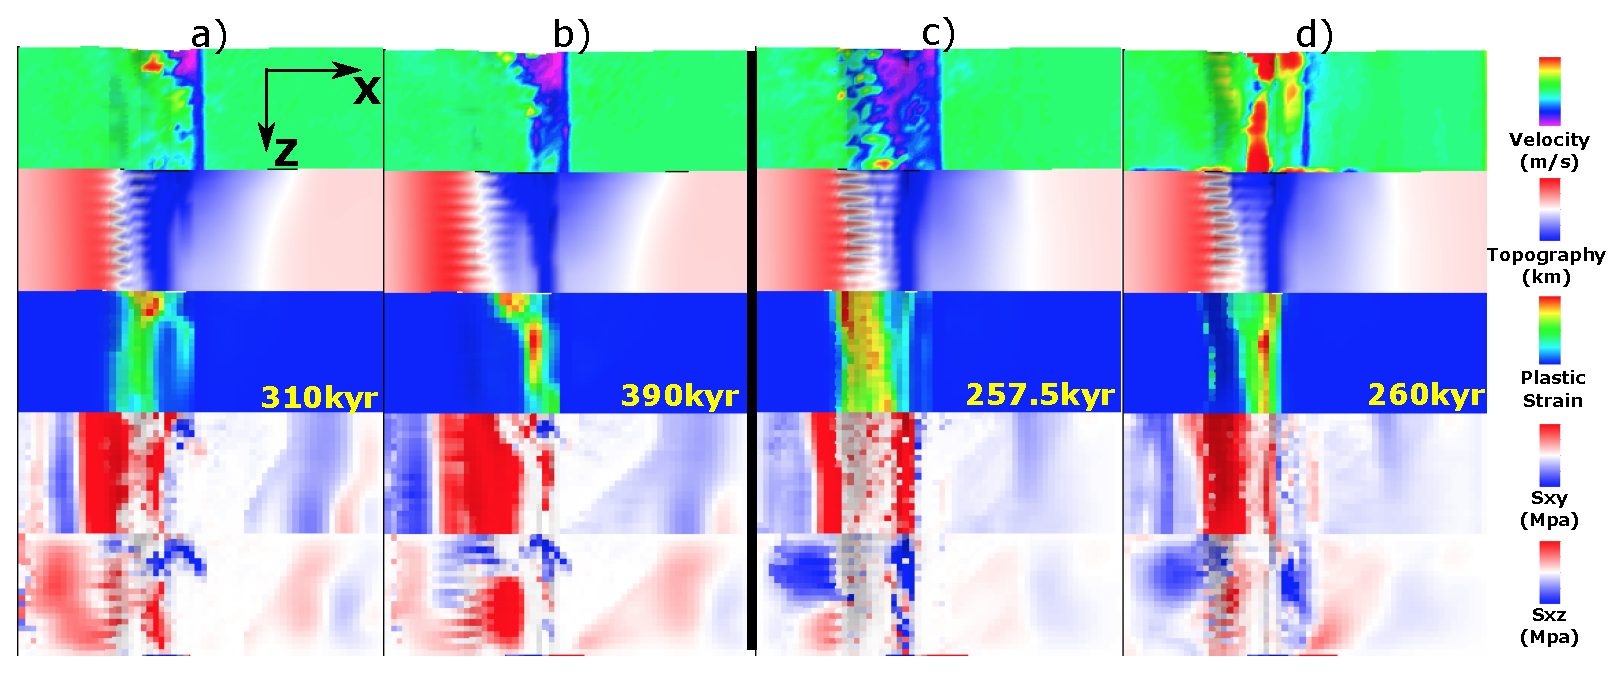
\includegraphics[width=1.0\textwidth]{fig_Results_Weakening_2_M57SinT1VST2_CutbackVSsecondaryFault.eps}
 \caption{M57SinT2 versus M57SinT1 (Table~\hyperref[Tab1_1]{\ref{Tab1_1}}). a) and b) are for M57SinT2, c) and d) are for M57SinT1.}
\label{fig_Results_Weakenging_2}
\end{figure}

Initially, both models develop normal fault deformations on both sides of the ridge-axis at the low M side. The time for the faults to propagate toward the high M side and cut through the whole crust for M57SinT1 (25kyr) is one half of that for M57SinT2 (50kyr). At around 310kyr, a near axis secondary fault begin to evolve for M57SinT2 at higher M side (Z$>5$) and soon take the place of initial fault, while at lower M side (Z$<=$5), the initial fault remains (Figure~\hyperref[fig_Results_Weakenging_2]{\ref{fig_Results_Weakenging_2}.a) and b)}). However, for M57SinT1, cut back happens around 260kyr and help to maintain a high angle fault with closer to ridge-axis termination. The initial fault remains, no secondary fault forming (Figure~\hyperref[fig_Results_Weakenging_2]{\ref{fig_Results_Weakenging_2}.a) and b)}). In addition, the width of median valley at low M side is wider for M57SinT2 than M57SinT1 (Figure~\hyperref[fig_Results_Weakenging_2]{\ref{fig_Results_Weakenging_2}.a) and b) versus c) and d)}) due to slower weakening (Type two) alows a more distributed tensional stress $\sigma_{xx}$ rather than fast weakening that once a fault is established, larger amount of tensional stress $\sigma_{xx}$ will be released at the fault.  

\begin{figure}[h]
 \centering
  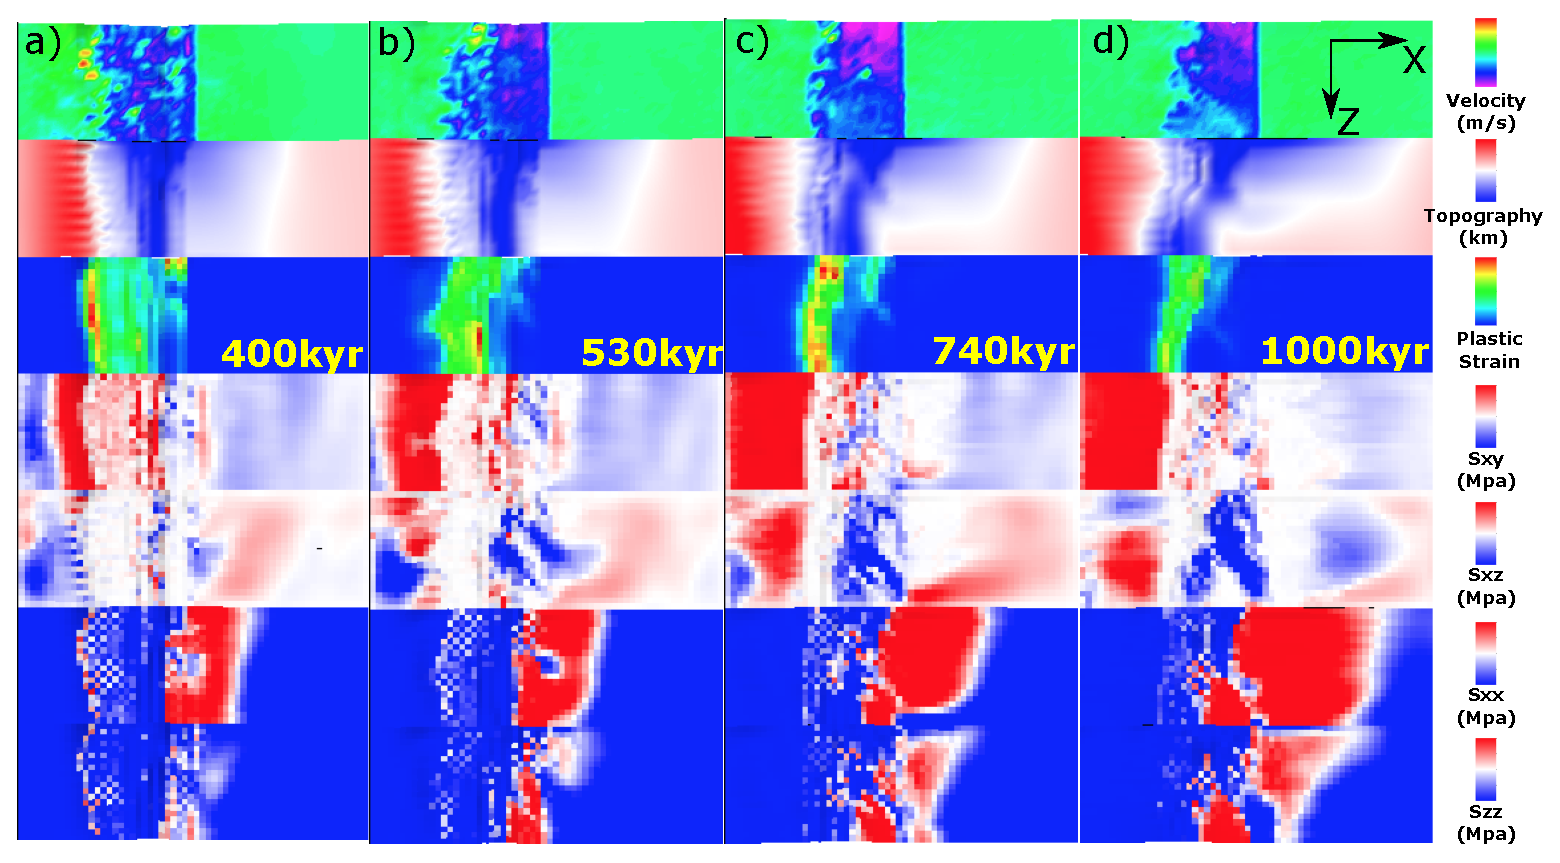
\includegraphics[width=1.0\textwidth]{fig_Results_Weakening_3_M57SinT1_time_evolution.eps}
 \caption{M57SinT1 (Table~\hyperref[Tab1_1]{\ref{Tab1_1}}) faulting and stress evolution with respect to time.}
\label{fig_Results_Weakenging_3}
\end{figure}

For M57SinT1, as shown in Figure~\hyperref[fig_Results_Weakenging_3]{\ref{fig_Results_Weakenging_3}}, at 400kyr (a), there is opposite dipping normal fault forming at the low M side accommodating part of the extension, which results in a curved termination at the far frontier. As it evolve (530kyr (b)), the termination at the low M side further recedes backward while the termination at the center (Z$=11\sim13$) extends further. This curved termination leads to a curved topography (white curve in the second row). As the fault evolve and bend further away from the axis, at the time of 740kyr, another opposite dipping normal fault forming again a the low M side (c). It doesn't take the place of initial fault and disapear soon, however, it again releases tensional stress and maintain the termination at far front recede backward. At 1000kyr(d), an Atlantiss Massif shape OCC is produced (low M side (lower magma supply) has a wider dome and high M side (higher magma supply) has a narrower dome) due to the along ridge-axis termination evolution. Corrugations with wavelength varying from hundreds to kilometers are also created.       

\begin{figure}[h]
 \centering
  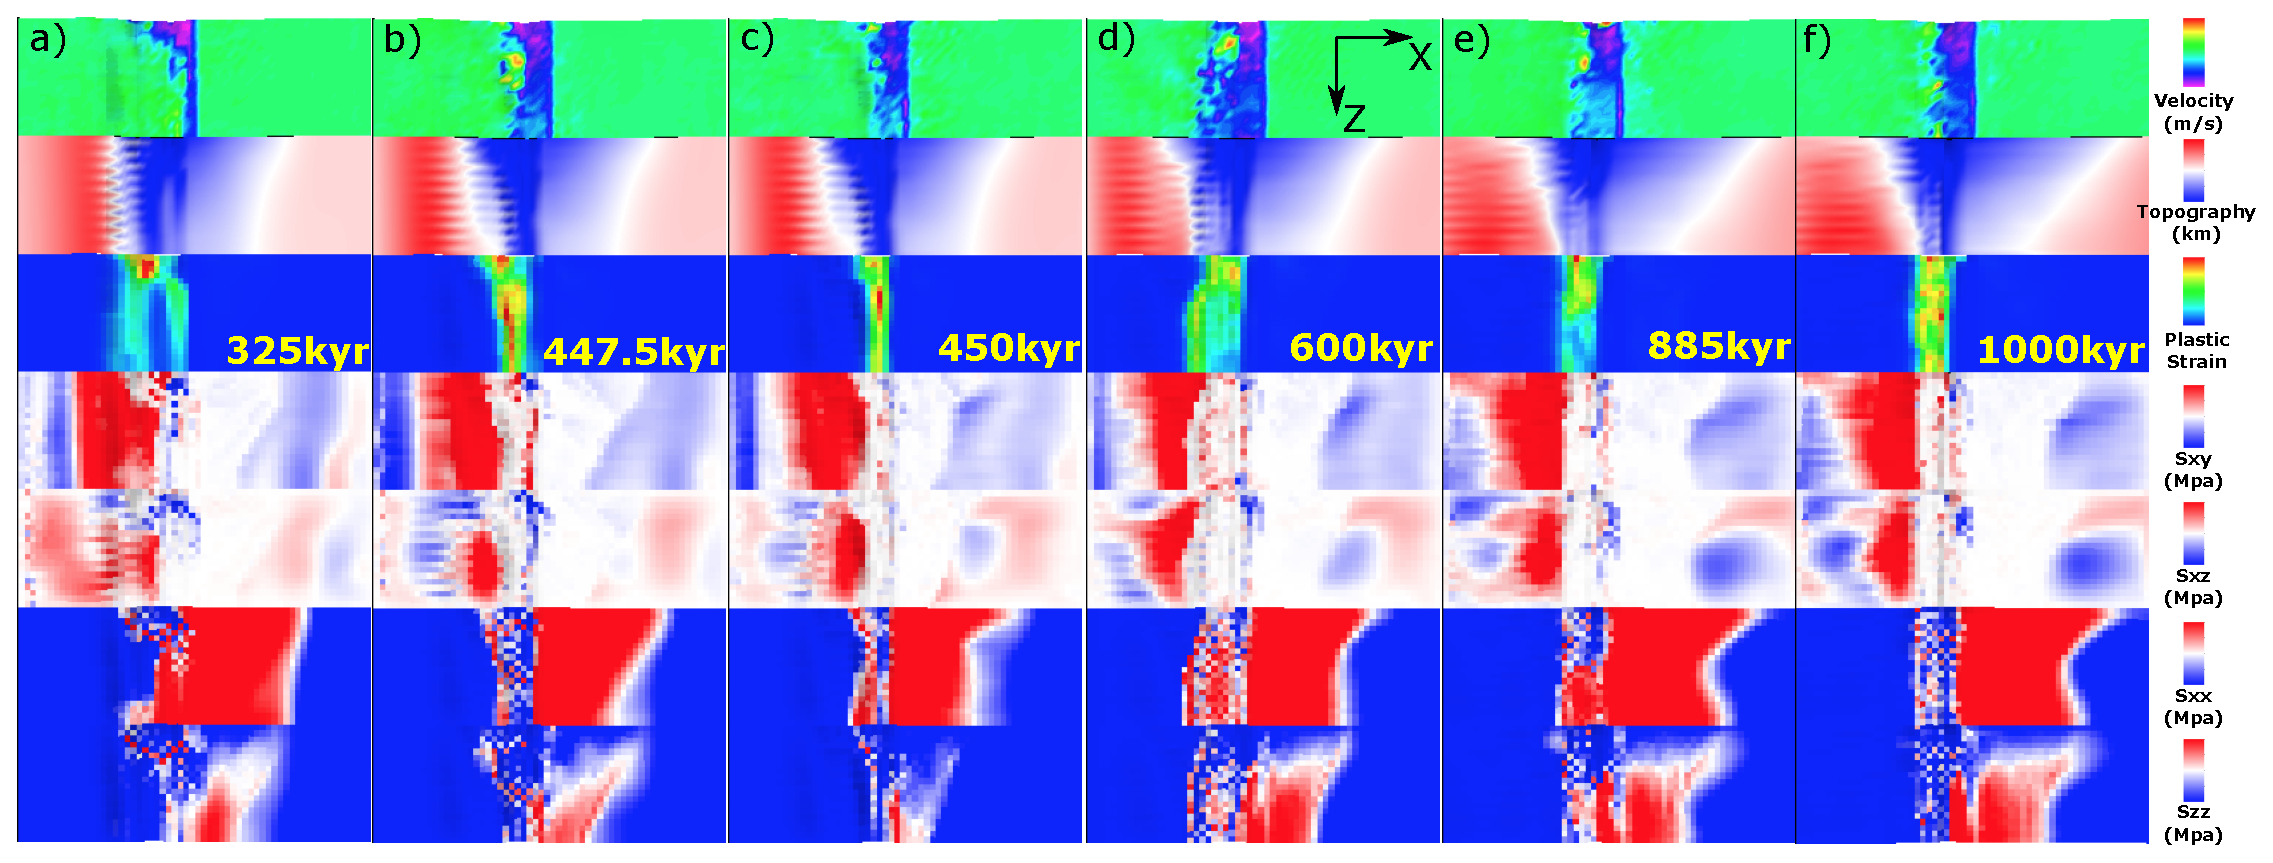
\includegraphics[width=1.0\textwidth]{fig_Results_Weakening_4_M57SinT2_time_evolution.eps}
 \caption{M57SinT2 (Table~\hyperref[Tab1_1]{\ref{Tab1_1}}) faulting and stress evolution with respect to time.}
\label{fig_Results_Weakenging_4}
\end{figure}

For M57SinT2, as shown in Figure~\hyperref[fig_Results_Weakenging_4]{\ref{fig_Results_Weakenging_4}}, instead of maintaining one fault all the time for M57SinT1, it creats secondary fault at high M side with different mechanism several times. A secondary fault is created at 325kyr (a), when a new near axis normal fault take the place of the initial one at high M side. Between 447.5kyr (b) and 450kyr (c), termination falls back, and as it evolve, termination at the high M side extends further at 600kyr (d). At 885kyr, a secondary fault propagates from low Z to high Z and terminates the further extended fault at high Z and maintain a near ridge-axis termination.

\subsubsection{M58SinT1 versus M58SinT2}

A major difference between M58SinT1 and M58SinT2 is that M58SinT1 keep faulting at one side of the ridge-axis while M58SinT2's fault alternates.

\begin{figure}[h]
 \centering
  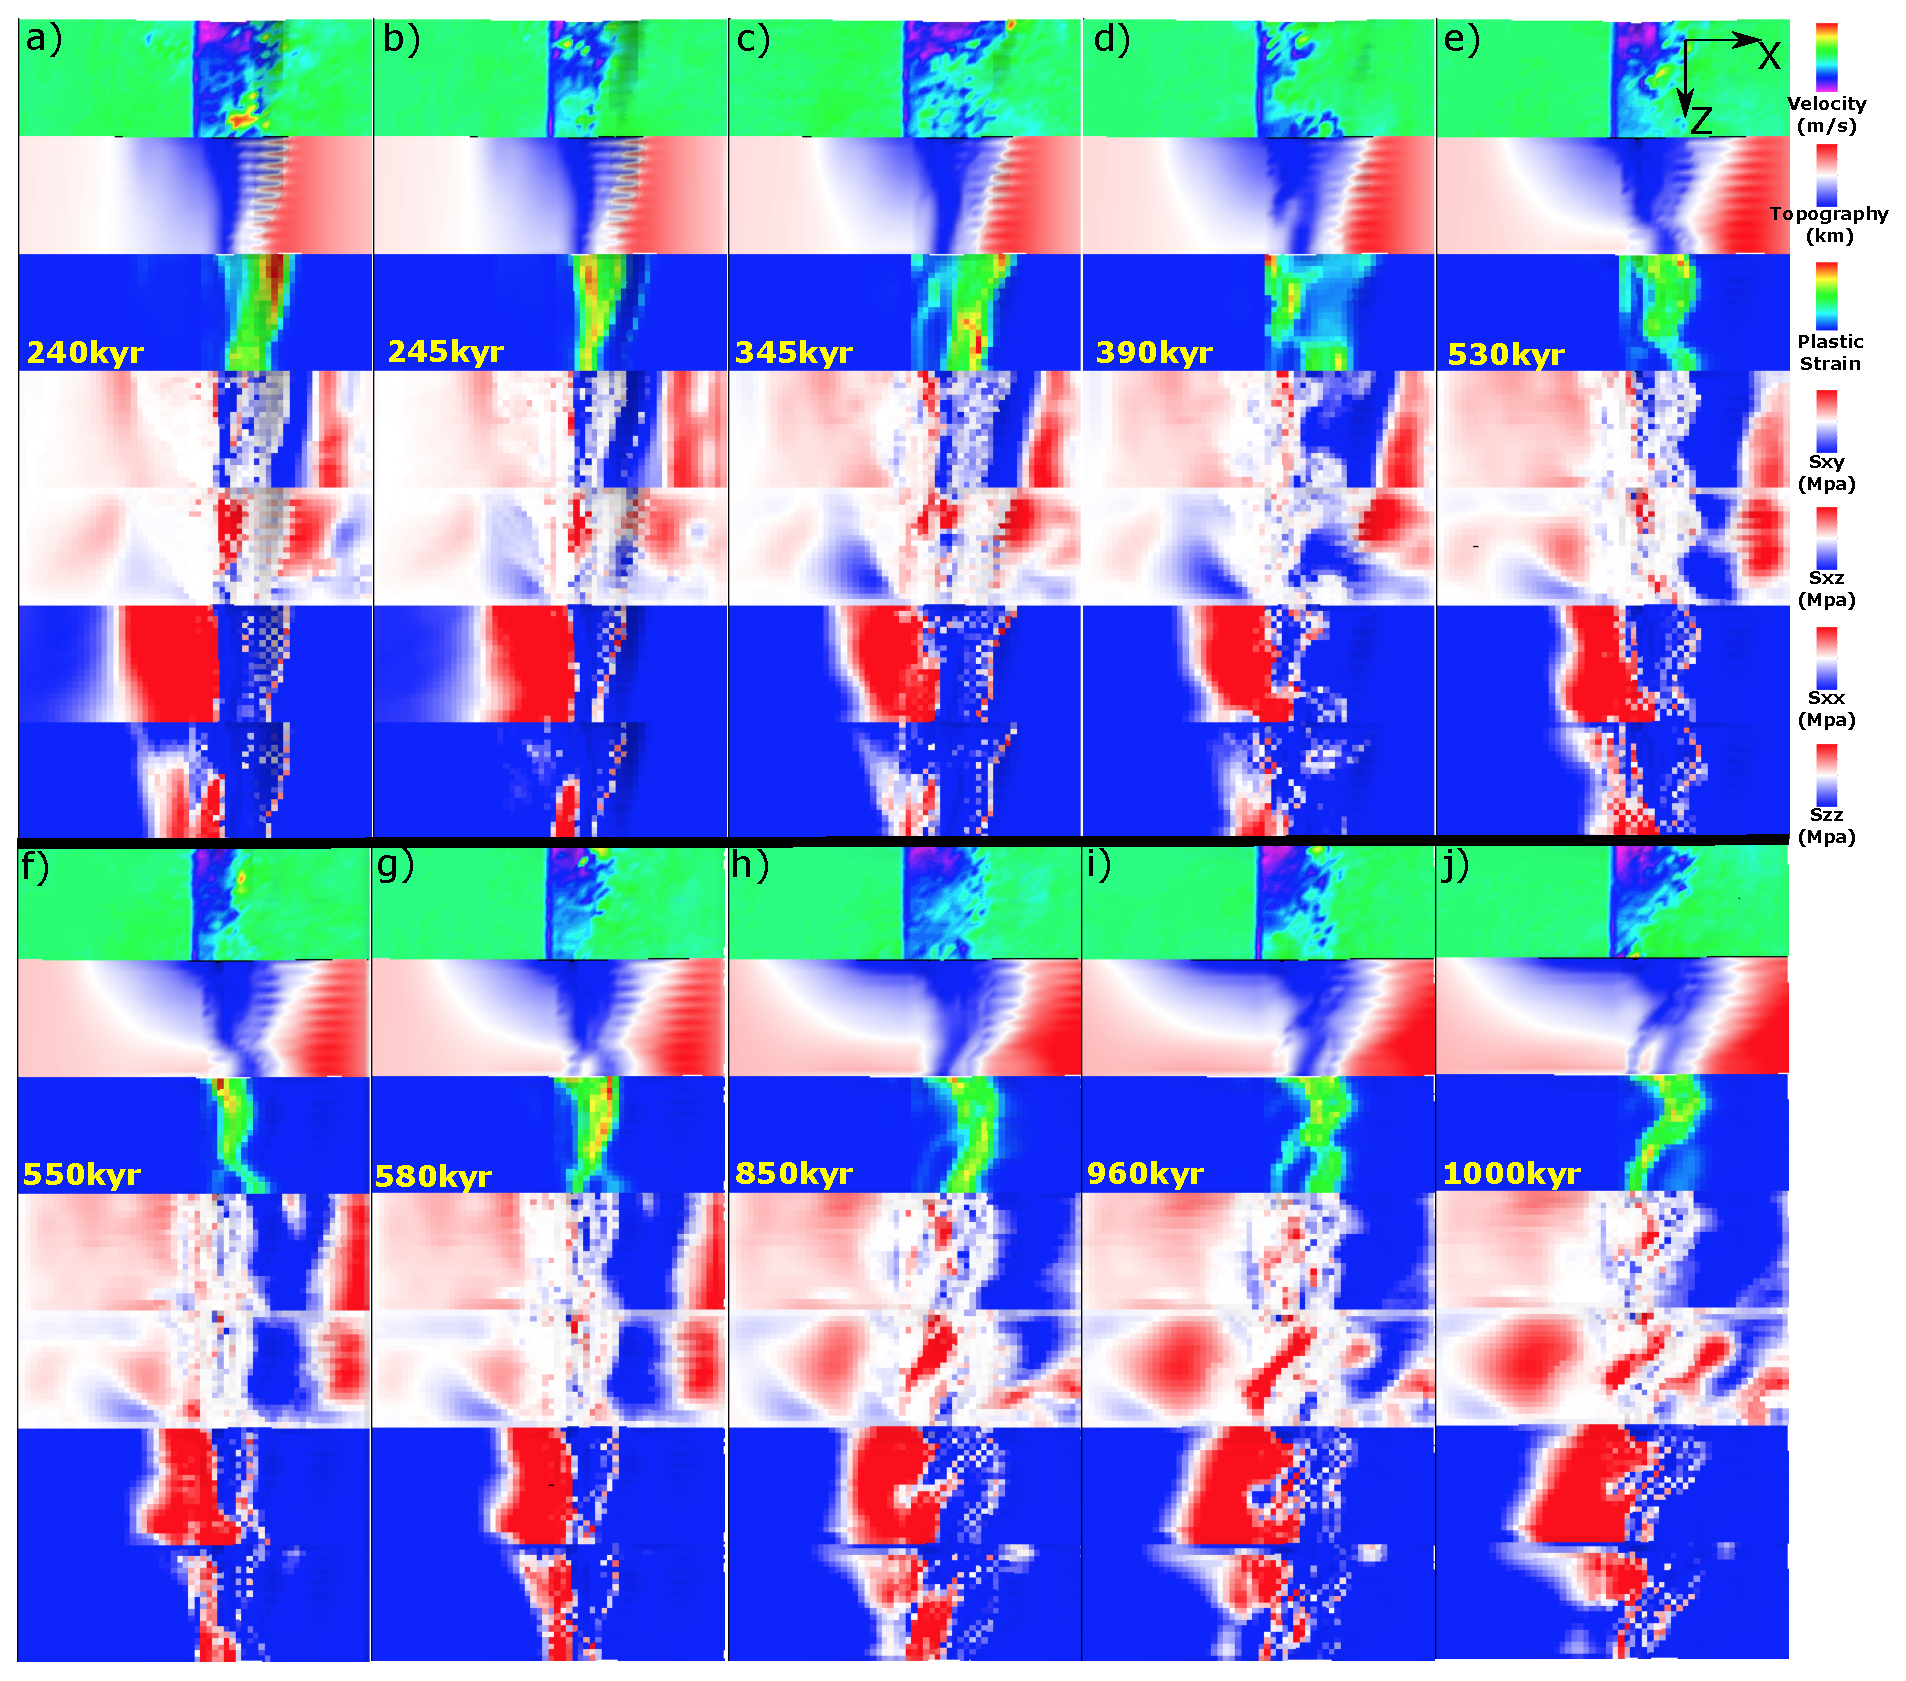
\includegraphics[width=1.0\textwidth]{fig_Results_Weakening_5_M58SinT1_time_evolution.eps}
 \caption{M58SinT1 (Table~\hyperref[Tab1_1]{\ref{Tab1_1}}) faulting and stress evolution with respect to time.}
\label{fig_Results_Weakenging_5}
\end{figure}

\paragraph{M58SinT1}
As shown in Figure~\hyperref[fig_Results_Weakenging_5]{\ref{fig_Results_Weakenging_5}}, in 1Myr, the fault keeps on the right hand side of the ridge-axis. It evolves dynamically. Between 240kyr (Figure~\hyperref[fig_Results_Weakenging_5]{\ref{fig_Results_Weakenging_5}.a}) and 245kyr (Figure~\hyperref[fig_Results_Weakenging_5]{\ref{fig_Results_Weakenging_5}.b}), there is a cut back. At 345kyr (Figure~\hyperref[fig_Results_Weakenging_5]{\ref{fig_Results_Weakenging_5}.c}), at low Z side, there are two offsetted antithetic faults (Z=$1\sim2$ and Z=$5\sim9$) in the hanging wall begin to evolve and soon connect to each other forming anastomosing fault zone. At 390kyr (Figure~\hyperref[fig_Results_Weakenging_5]{\ref{fig_Results_Weakenging_5}.d}), the new near axis anastomosing fault zone replace the old further away from ridge-axis detachment. There is dextral $\sigma_{xz}$ forming on the right hand side of the new anastomosing fault zone ((Figure~\hyperref[fig_Results_Weakenging_5]{\ref{fig_Results_Weakenging_5}.d}), row 5) due to the offset between the new near axis fault at low Z side and extended further fault at high Z side and leads to the development of a $\sim45\degree$ shear zone connection between the new near axis fault zone at low Z side and the further away from axis original detachment at high Z side. It also creates a curved termination which will lead to a curved topography (boundary between blue and white) seen at 530kyr (Figure~\hyperref[fig_Results_Weakenging_5]{\ref{fig_Results_Weakenging_5}.e}). Note that this curved termination can be a mechanism for producing large wavelength (several kilometers) undulating corrugations. Between 530kyr (Figure~\hyperref[fig_Results_Weakenging_5]{\ref{fig_Results_Weakenging_5}.e}) and 550kyr (Figure~\hyperref[fig_Results_Weakenging_5]{\ref{fig_Results_Weakenging_5}.f}), there is another cut back happens. Terminations fall backwards to near ridge-axis position. At 580kyr (Figure~\hyperref[fig_Results_Weakenging_5]{\ref{fig_Results_Weakenging_5}.g}), at the high Z side, a new near rigde-axis high angle normal fault begin to initiate under the assistance of rotational force from low Z side due to along ridge-axis coupling. This produces a large rider block with several kilometers in its length scale. Previous ``S'' curved termination now evolves to a half circle curve and it soon affects the curve of topography as seen at 850kyr (Figure~\hyperref[fig_Results_Weakenging_5]{\ref{fig_Results_Weakenging_5}.h}). Due to along ridge-axis variation in diking, a large sinistral shear zone (red region $\sim40\degree$ oblique to ridge axis seen in 5th row of 960kyr (Figure~\hyperref[fig_Results_Weakenging_5]{\ref{fig_Results_Weakenging_5}.i})) keep developing and cut the circle curved fault zone at 850kyr (Figure~\hyperref[fig_Results_Weakenging_5]{\ref{fig_Results_Weakenging_5}.h}) into a new fault zone with higher curvature as seen in 1000kyr (Figure~\hyperref[fig_Results_Weakenging_5]{\ref{fig_Results_Weakenging_5}.j}).         

\begin{figure}[h]
 \centering
  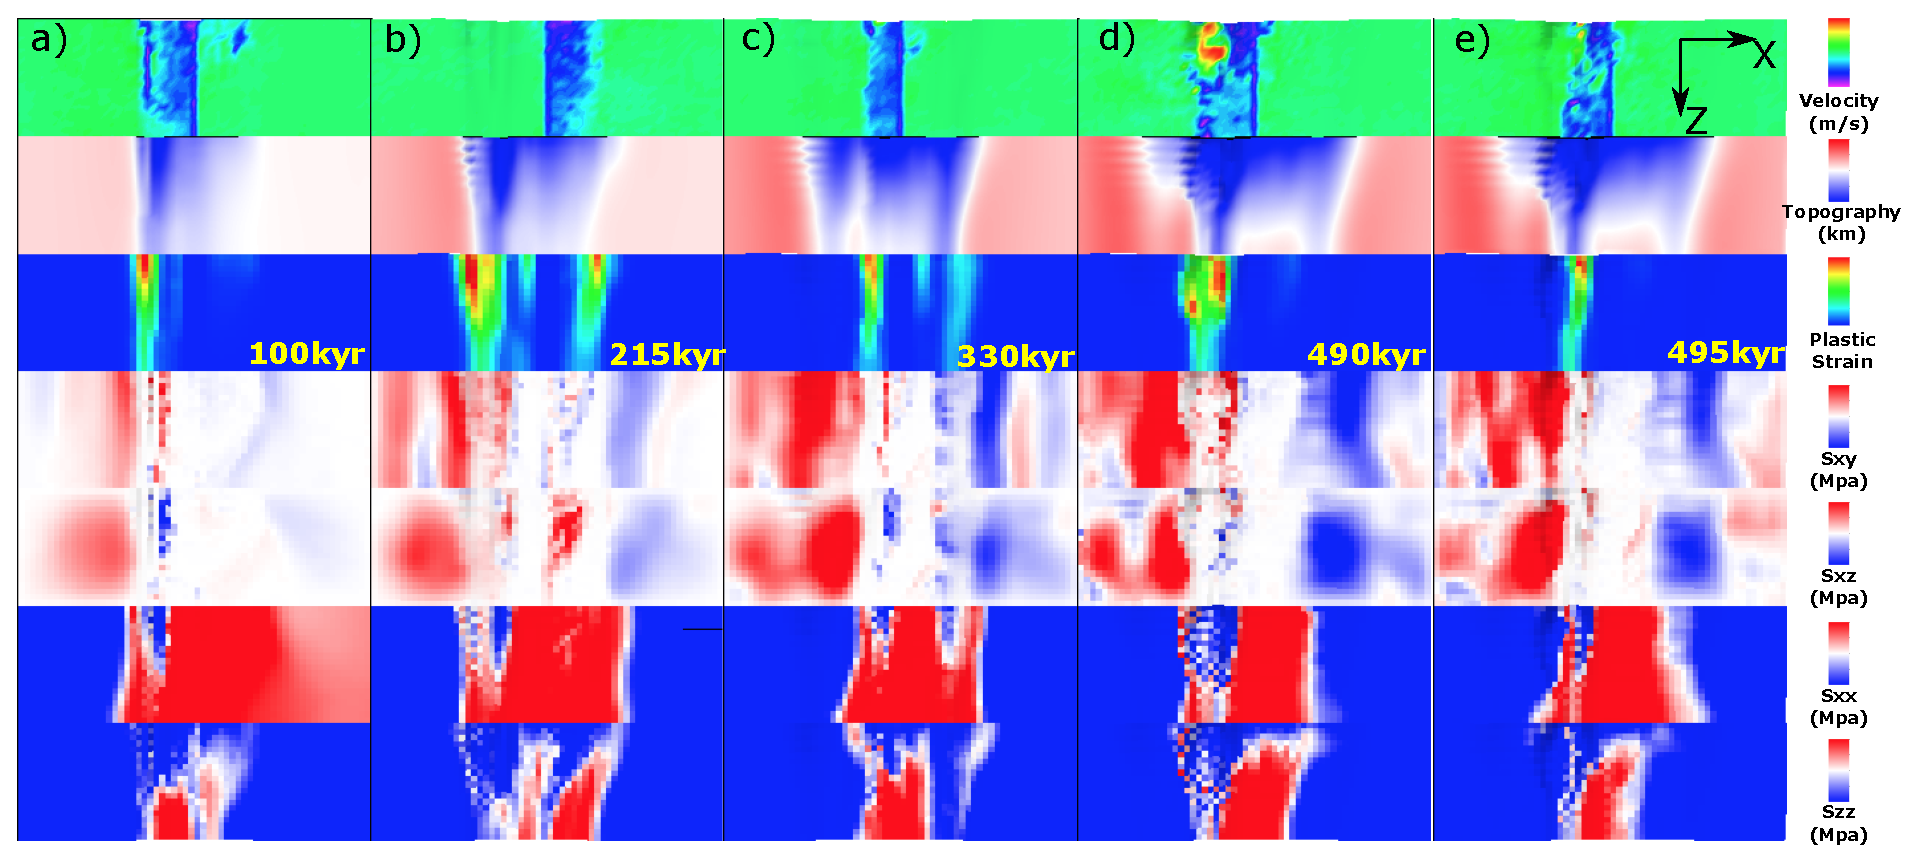
\includegraphics[width=1.0\textwidth]{fig_Results_Weakening_6_M58SinT2_time_evolution.eps}
 \caption{M58SinT2 (Table~\hyperref[Tab1_1]{\ref{Tab1_1}}) faulting and stress evolution with respect to time.}
\label{fig_Results_Weakenging_6}
\end{figure}

\paragraph{M58SinT2}
As shown in Figure~\hyperref[fig_Results_Weakenging_6]{\ref{fig_Results_Weakenging_6}}, the fault initiate on the left hand side of the ridge-axis (Figure~\hyperref[fig_Results_Weakenging_6]{\ref{fig_Results_Weakenging_6}.a}). Low Z side extends further than high Z side. It takes around 100kyr to form into a localized fault plane due to slower rate of weakening. At 215kyr (Figure~\hyperref[fig_Results_Weakenging_6]{\ref{fig_Results_Weakenging_6}.b}), another fault on the conjugate plate begin to evolve and replaces the initial one. As seen from (Figure~\hyperref[fig_Results_Weakenging_6]{\ref{fig_Results_Weakenging_6}.b}), corrugations are created at low Z side. At 330kyr, a third fault forming at the left hand side of the ridge-axis. Between 490kyr (Figure~\hyperref[fig_Results_Weakenging_6]{\ref{fig_Results_Weakenging_6}.d}) and 495kyr (Figure~\hyperref[fig_Results_Weakenging_6]{\ref{fig_Results_Weakenging_6}.e}), there is a cut back.

\subsubsection{M58SqrtT1 versus M58SqrtT2}
The major difference between M58SqrtT1 and M58SqrtT2 is also whether the normal fault alternates or not.
\paragraph{M58SqrtT1}

As shown in Figure~\hyperref[fig_Results_Weakenging_7]{\ref{fig_Results_Weakenging_7}}, initially, there is a 5 element offset between breakaways along the ridge-axis due to along ridge-axis variation in diking (Figure~\hyperref[fig_Results_Weakenging_7]{\ref{fig_Results_Weakenging_7}.a}). At 370kyr (Figure~\hyperref[fig_Results_Weakenging_7]{\ref{fig_Results_Weakenging_7}.b}), there is a vertical tensile failure at Z$=1\sim2$. Two parallel dextral (blue) shear regions are seen (5th row). The low Z shear zone assists in the shear failure observed at 400kyr (Figure~\hyperref[fig_Results_Weakenging_7]{\ref{fig_Results_Weakenging_7}.c}), and it develops into near ridge-axis normal fault (Z=$4\sim12$) and propagates to high Z side which eventually cuts through and reaches Z$=20$ and replaces the initial extended fault at high Z side at 460kyr (Figure~\hyperref[fig_Results_Weakenging_7]{\ref{fig_Results_Weakenging_7}.d}). The vertical tensile failure zone at Z$=1\sim3$ (Figure~\hyperref[fig_Results_Weakenging_7]{\ref{fig_Results_Weakenging_7}.d} 3rd row) begin to evolve and assists in the initiation of a new near ridge-axis high angle normal fault which connect with the fault at the high Z side (Figure~\hyperref[fig_Results_Weakenging_7]{\ref{fig_Results_Weakenging_7}.e}) at 590kyr. At 660kyr (Figure~\hyperref[fig_Results_Weakenging_7]{\ref{fig_Results_Weakenging_7}.f} 3rd row), there is a hint of high angle normal faulting at Z$=1\sim3$ of conjugate plate. But it doesn't develop. At 730kyr (Figure~\hyperref[fig_Results_Weakenging_7]{\ref{fig_Results_Weakenging_7}.g} 5th row), a dextral (blue) shear zone at the low Z side help to create the faulting pattern seen at 780kyr (Figure~\hyperref[fig_Results_Weakenging_7]{\ref{fig_Results_Weakenging_7}.h} 3rd row), a concave termination with a wavelenth of 10 kilometers and it has the potential to create a large wavelength corrugation. Meanwhile, at the low Z side, near the ridge-axis, there is a antithetic fault forming at the hanging wall of the detachment and it later propagates to high Z side (Figure~\hyperref[fig_Results_Weakenging_7]{\ref{fig_Results_Weakenging_7}.i}). From 820kyr to 880kyr, the antithetic fault evolves to near ridge-axis normal fault and connects with the detachment at the high Z side (Figure~\hyperref[fig_Results_Weakenging_7]{\ref{fig_Results_Weakenging_7}.j}). In addition, a tensile failure shows its hint at the low Z side (Z$=1\sim5$) of the conjugate plate.         

\begin{figure}[h]
 \centering
  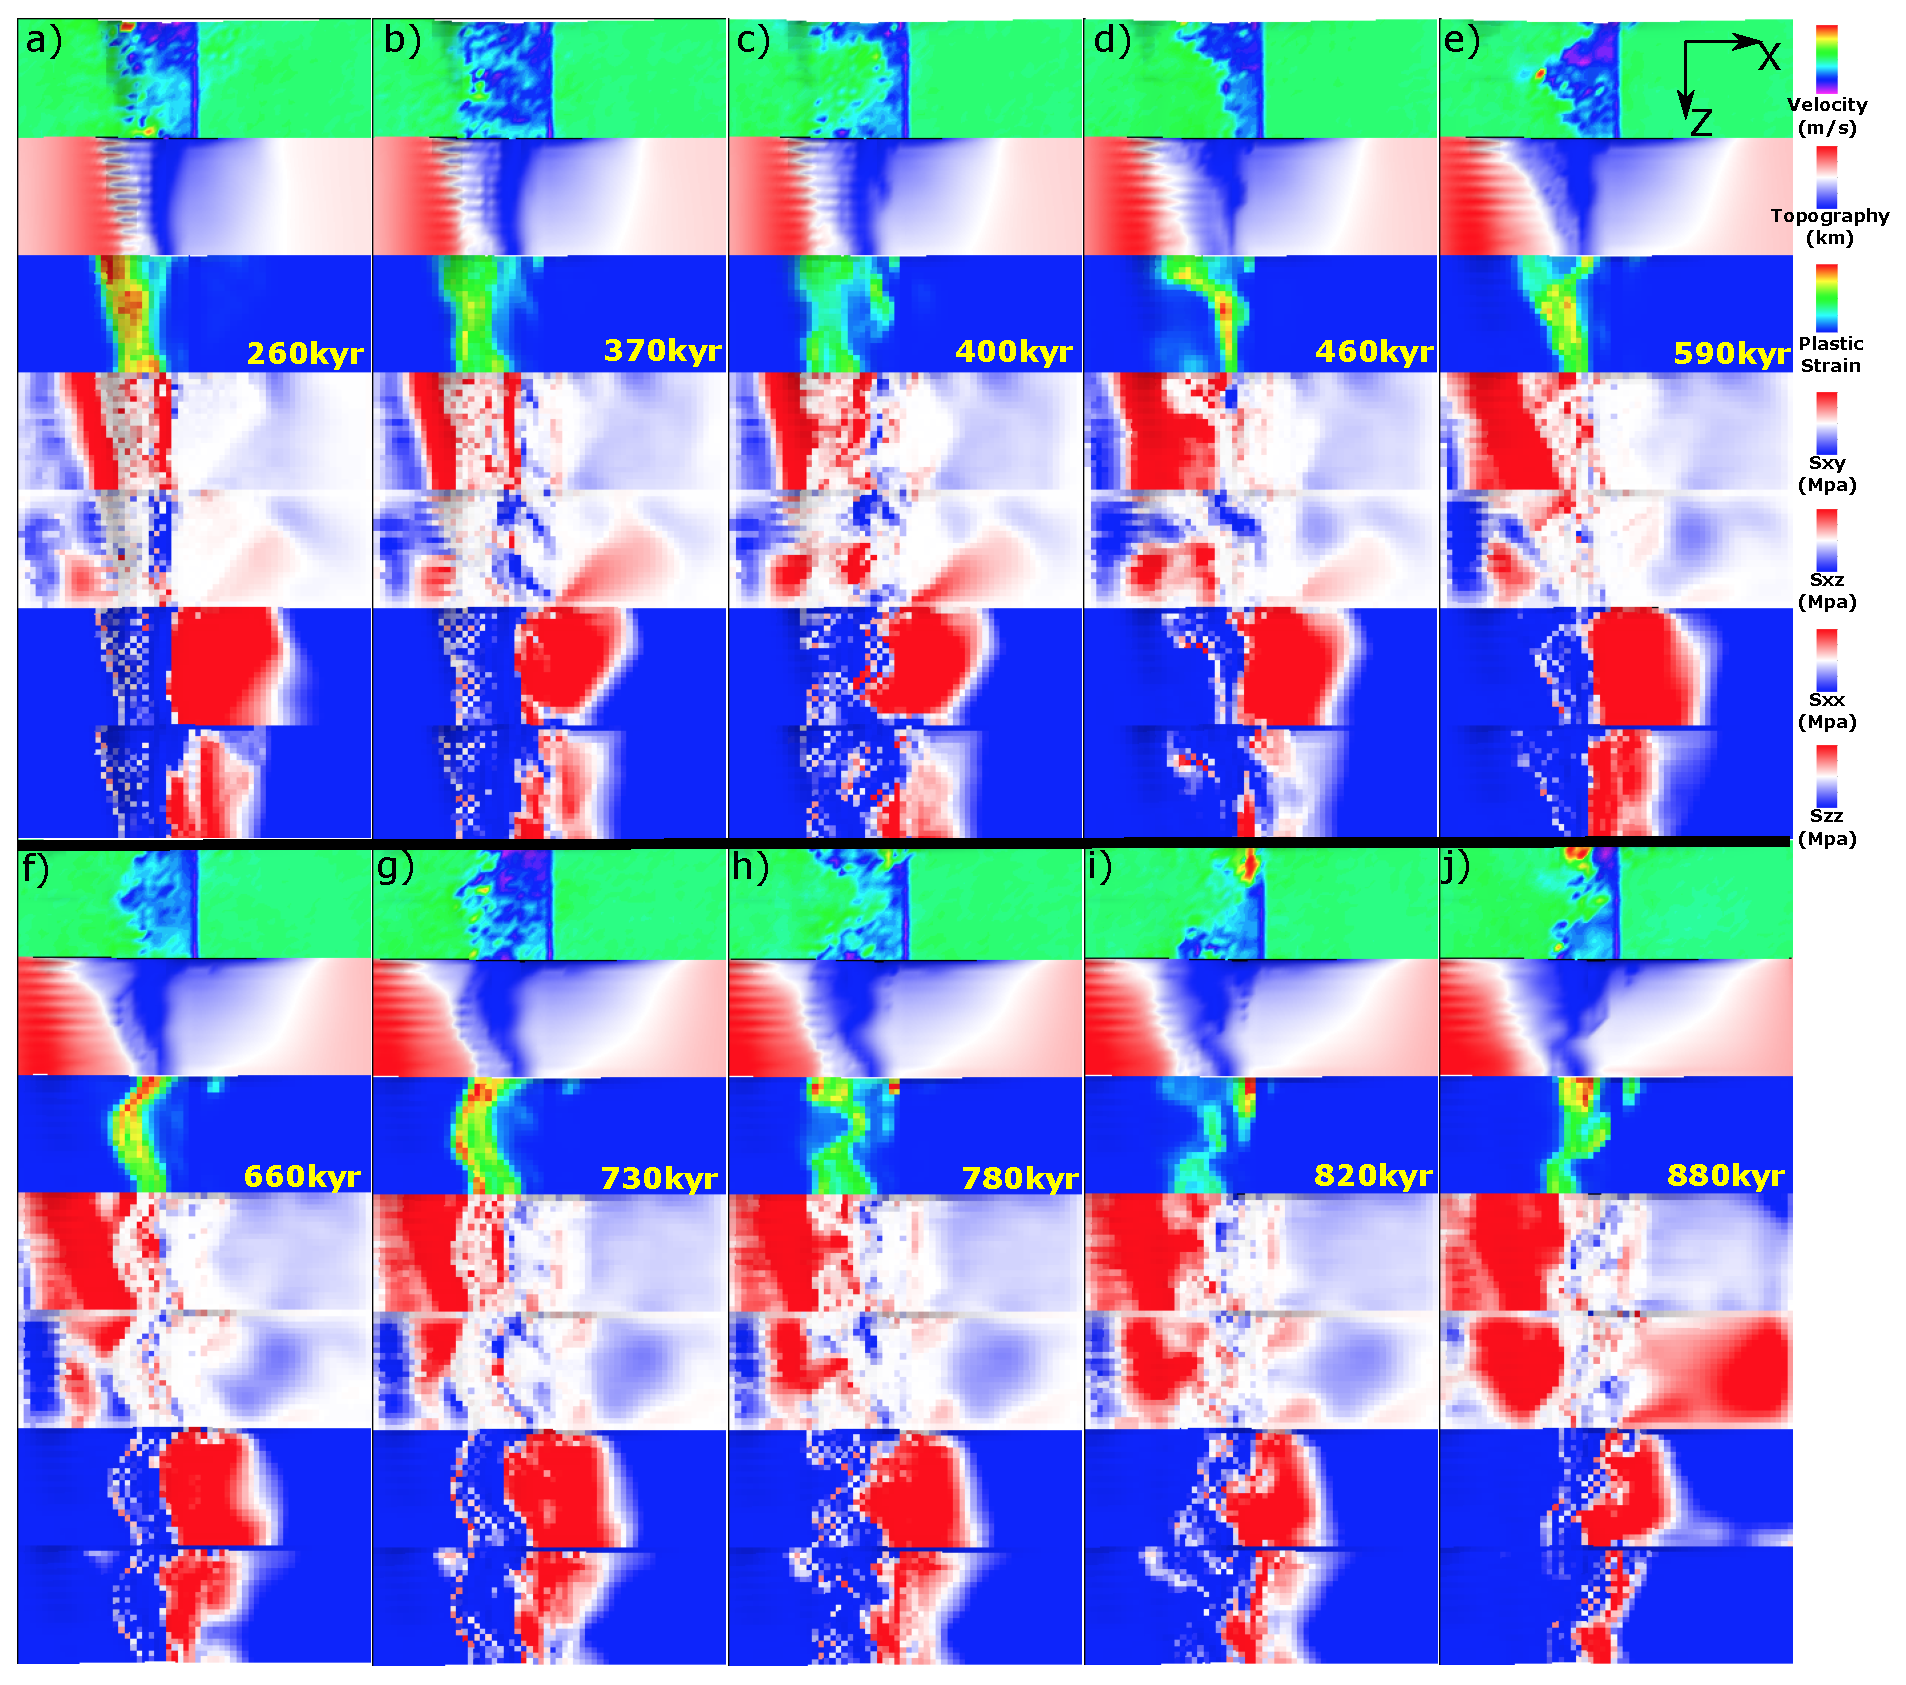
\includegraphics[width=1.0\textwidth]{fig_Results_Weakening_7_M58SqrtT1_time_evolution.eps}
 \caption{M58SqrtT1 (Table~\hyperref[Tab1_1]{\ref{Tab1_1}}) faulting and stress evolution with respect to time.}
\label{fig_Results_Weakenging_7}
\end{figure}

\paragraph{M58SqrtT2}

\begin{figure}[h]
 \centering
  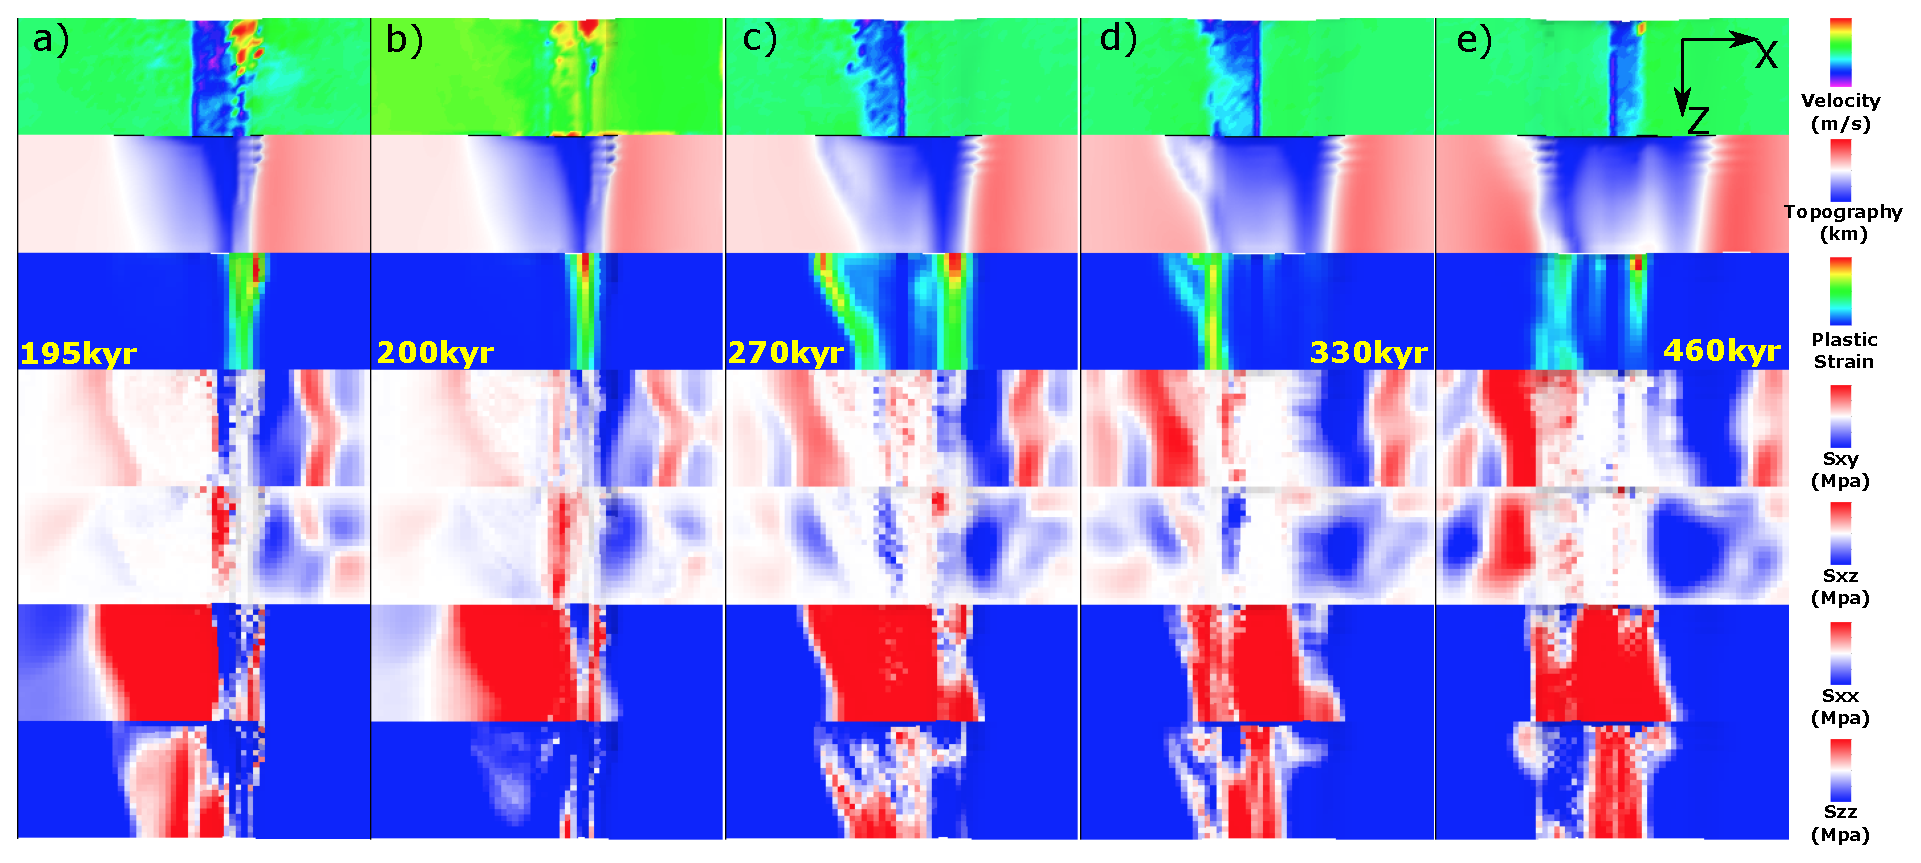
\includegraphics[width=1.0\textwidth]{fig_Results_Weakening_8_M58SqrtT2_time_evolution.eps}
 \caption{M58SqrtT2 (Table~\hyperref[Tab1_1]{\ref{Tab1_1}}) faulting and stress evolution with respect to time.}
\label{fig_Results_Weakenging_8}
\end{figure}

As shown in Figure~\hyperref[fig_Results_Weakenging_8]{\ref{fig_Results_Weakenging_8}}, 

\subsection{Variation of the range of M}
We have three ranges for M variation along the ridge-axis: M28, M57 and M58 (M28 means M varies from 0.2 to 0.8 from front to end as Z increases). Among the 12 available models, two M58 models and the constant M$=0.8$ model with Type two weakening produce fault alternation while others do not. Generally, M57 and M58 models create a median valley much narrower and shallower.

\subsubsection{Fault Alternation}
The fault alternation behavior observed in pseudo-2D models in cases M$>0.5$ is much more complicated in 3D models. The results shows that only Type two weakening with M58 will result in a alternating faulting pattern. \add[XT]{integrate the area of M$>0.5$ with respect to Z to see if there is any quantatative analysis available.}

\subsection{Corrugations}
The stress at the tips of the breakaways is generally tensional in both parallel and orthogonal directions to the ridge-axis. (Figure~\hyperref[fig_Results4_3_1]{\ref{fig_Results4_3_1}.f,g})


\subsubsection{Wavelength of corrugations}

\subsection{Summary of Findings}
